%------ LaTeX-Template für Abschlussarbeiten, Prof. Thomas Görne, Dezember 2012 --------
%------ Modified by B.Sc. Julius Neudecker, May 2021 ------

%---- Header (mit Formateinstellugen) laden, Inputencoding prxfen ------

%%%%%%%%%%%%%%%%%%%%%%%%%%%%%%%%%%%%%%%%%%%%%%%%%
%---- LaTeX-Header fuer Abschlussarbeiten, Prof. Thomas Goerne, Dez. 2012/Aug. 2013 ----
%------ Modified by B.Sc. Julius Neudecker, May 2021 ------
%%%%%%%%%%%%%%%%%%%%%%%%%%%%%%%%%%%%%%%%%%%%%%%%%

\documentclass[12pt,paper=A4,pointlessnumbers,bibtotoc,liststotoc,DIV=11,BCOR=1mm]{scrreprt}
% BCOR ist die Bindekorrektur (verlorener Rand am linken Blattrand)! Wert haengt von der Art der Heftung ab!!
% DIV ist eine Satzspiegeleinstellung von KOMA-Script / sccreprt.

\pagestyle{headings}

\usepackage[T1]{fontenc} % Font Encoding fuer europaeische Schriften mit Umlauten (Unterstuetzung der Worttrennung)
\usepackage{lmodern} % PostScript-Varianten der TeX Computer Modern-Schriften laden
\usepackage[english]{babel} % Spracheinstellungen fuer Englisch und Neudeutsch laden

\usepackage{graphicx} % Grafikeinbindung (fuer .JPG, .JPEG, .PNG und .PDF, falls pdflatex benutzt wird)
\usepackage[table]{xcolor} % ermoeglicht farbige Schrift und farbige Tabellenzeilen
\definecolor{black}{gray}{0} % Umdefinition der Farbe black, falls noetig (0=schwarz, 1=weiss)
\definecolor{dblue}{rgb}{0.1,0.2,0.6} % Dunkelblau, fuer Hyperlinks
\definecolor{lgray}{gray}{0.9} % Hellgrau, fuer Tabellen (0=schwarz, 1=weiss)

\usepackage{booktabs} % fuer schoene Tabellen

\usepackage[round,authoryear]{natbib} % Literaturverweise mit Name/Jahreszahl in runden Klammern
\bibpunct[:\,]{(}{)}{,}{a}{}{,~}  % Feinformatierung der Natbib-Zitierweise

\usepackage[hyphens]{url}
\usepackage[colorlinks=true,linkcolor=black,citecolor=dblue,urlcolor=dblue]{hyperref} 
\usepackage{hyperref}  
% die Pakete url und hyperref ermoeglichen anklickbare URLs im Quellenverzeichnis in definierter Farbe, 
% sie ermoeglichen den Zeilenumbruch bei langen URLs, und sie erzeugen Hyperlinks (Farbe s.o.) 
% zwischen Quellenverweis und Quellenverzeichnis sowie zwischen label und ref im PDF-Dokument

% Fonteinstellungen fuer Bildunterschriften: Unterschrift serifenlos, "Abbildung" fett (bfseries = bold face series)
\setkomafont{captionlabel}{\sffamily\bfseries}
\setkomafont{caption}{\sffamily}

% Ordner für Grafiken
\graphicspath{ {./images/} }

%% ToDo Notes
\newcommand\todo[1]{\textcolor{red}{#1}}

%------------------------------------------------------------------------------------------------------------------
%------ Eigenstaendigkeitserklaerung im gerahmten Kasten (parbox in einer framebox) ------
%------------------------------------------------------------------------------------------------------------------

\newcommand{\eigen}{
\setlength{\fboxsep}{2ex}
\setlength{\fboxrule}{0.8pt} 
% Einstellungen fuer Rahmenabstand und Rahmendicke der Framebox
\begin{center}
	\fbox{
		\parbox{0.8\linewidth}{
			I hereby confirm that this thesis is my own work and that I have not sought or used inadmissible help of third parties to produce this work and that I have clearly referenced all sources used in this thesis. I have fully referenced and used inverted commas for all text directly or indirectly quoted from a source.
		\par\bigskip\bigskip\bigskip\bigskip
		\hspace*{0.8cm}Place and date \hfill \vorname~\nachname\hspace*{0.8cm}
		}
	}
\end{center}
}

%%%%%%%%%%%%%%%%%%%%%%%%%%%%%%%%%%%%%%%%%%%%%%%%%

\usepackage[utf8]{inputenc} % Inputencoding, universell

%------------------------ Titelblatt-Layout laden ----------------------------------

%%%%%%%%%%%%%%%%%%%%%%%%%%%%%%%%%%%%%%%%%%%%%%%%%
%------ LaTeX-Titelblatt fuer Bachelorarbeiten, Prof. Thomas Goerne, Dezember 2012 -------
%------------------------------------------------------------------------------------------------------------------
%--------------------------------- Deklarationen fuer die Titelseite  --------------------------------------
%%%%%%%%%%%%%%%%%%%%%%%%%%%%%%%%%%%%%%%%%%%%%%%%%

\title{\titel\\[2ex]
\LARGE Masters Thesis\\
\large To obtain the academic degree M.Sc.\\[1.5ex]
\LARGE \vorname~\nachname\\[0.5ex] 
\large \matrikelnummer
}

\author{\unitlength1mm
\large\raisebox{-1ex}{
\includegraphics[width=4em]{HAW_wuerfel}}\hspace{1ex}
\parbox[b]{11.2cm}{\sffamily\large%
University of applied sciences Hamburg\\[-0.2ex]
Faculty of Design, Media und Information\\[-0.2ex]
Department of Media Engineering
}\\[6ex]
\sffamily\large First examiner: \erstpruef\\[0.5ex]
\sffamily\large Second examiner: \zweitpruef}

%%%%%%%%%%%%%%%%%%%%%%%%%%%%%%%%%%%%%%%%%%%%%%%%%

%---------------------------- Titeldefinitionen --------------------------------------

\newcommand{\vorname}{Julius}
\newcommand{\nachname}{Neudecker}
\newcommand{\matrikelnummer}{2025850}

\newcommand{\titel}{{The influence of age on the ability to use Brain-Computer-Interfaces}\\[0.2ex] 
				\Large use case: TV remote control}

\newcommand{\erstpruef}{Prof. Dr.Roland Greule}
\newcommand{\zweitpruef}{Dipl. Inf. Rüdiger Höfert}

\date{preliminary version from \today}   % praktisch fxr Vorab-Versionen. 
%\date{\sffamily Hamburg, 30.06.2021}  % Abgabedatum!

%--------------------------------------------------------------------------------------
%----------------------------- hier gehts los! --------------------------------------
%--------------------------------------------------------------------------------------

\begin{document}
    \selectlanguage{english}
    \maketitle
    \tableofcontents
    \clearpage          % Seitenumbruch

    %------------ Zusammenfassung / Abstract ------------------

    \thispagestyle{empty}
    \selectlanguage{english}
    \section*{\centering\abstractname}
    In recent years, Brain Computer Interfaces - BCI in short - evolved to a level of maturity which allows for these devices to be produced cheaply and thus being available to consumers. This study used a device from a manufacturer called \textit{NextMind} to examine whether age has an effect on the ability to use such a device. A study was carried out with 30 participants from different age groups. They were confronted with a task where they had to use a graphical user interface which represented a remote control. Selecting elements was achieved by looking at them and the BCI recognized the target by means of SSVEP evaluation. The goal was to select a visually highlighted element as fast as possible in order to reach good results. The study showed that in fact age does have an impact on the overall performance by showing that people above the age of 40 exhibited a statistically significant longer detection time. Other factors were also examined but these did not show an effect which was unrelated to age.

    \chapter{Introduction}\label{introduction}

        In recent years significant progress has been made on the development of interfaces which relies on direct interaction with the brain itself. The latest popular example is Elon Musk's \textit{Neuralink} with their monkey learning to play the game \textit{Pong} only by using its brain (\cite{Neuralink.2021}). Apart from a solid scientific methodology, this study also presented a good media coverage including a showcase video which went viral. However there are more examples of a working interface, which will be discussed in section \ref*{related-work}, since this vast area of research is an intersection between several areas of research: medical engineering, neuroscience, computer science and HCI\footnote{Human Computer Interaction}.
        These interfaces are generally called \textit{Brain-Computer-Interface} or \textit{BCI} in short. \cite{MicrosoftResearch.23102020} has a very precise definition of the scope:

        \medskip
            \emph{Brain-Computer Interface (BCI) is a system that measures central nervous system (CNS) activity and converts it into artificial output that replaces, restores, enhances, supplements, or improves the natural CNS output and thereby changes the ongoing interactions between the CNS and its external or internal environment. BCI is direct communication pathway between an enhanced or wired brain and an external device.}
        \medskip

        As of Q2 2021 there are already devices available for consumers to buy, which fall into this category. This opens up possibilities for a widespread application of these kind of interfaces. Nevertheless, new ways of interacting with computers require some degree of research to define useful and user-friendly ways to interact with such technology. This study aims to provide insight into one aspect of this process.

        After a thorough disussion about the state of research in this field, the research hypothesis will be defined based on considerations about future use cases. Subsequently a user survey will be designed, carried out and conclusively evaluated to put the results into context.

        \clearpage\thispagestyle{empty}
        
        \section{Management Summary}

            In the \textit{2018 Gartner Hype Cycle} report (\cite{Gartner.24052021}), which is shown in figure \ref*{gartner-2018}, BCIs are denoted as to be on the brink of the peak of inflated expectations:

            \begin{figure}[h]     % h=here, t=top, b=bottom, p=page
                \centering
                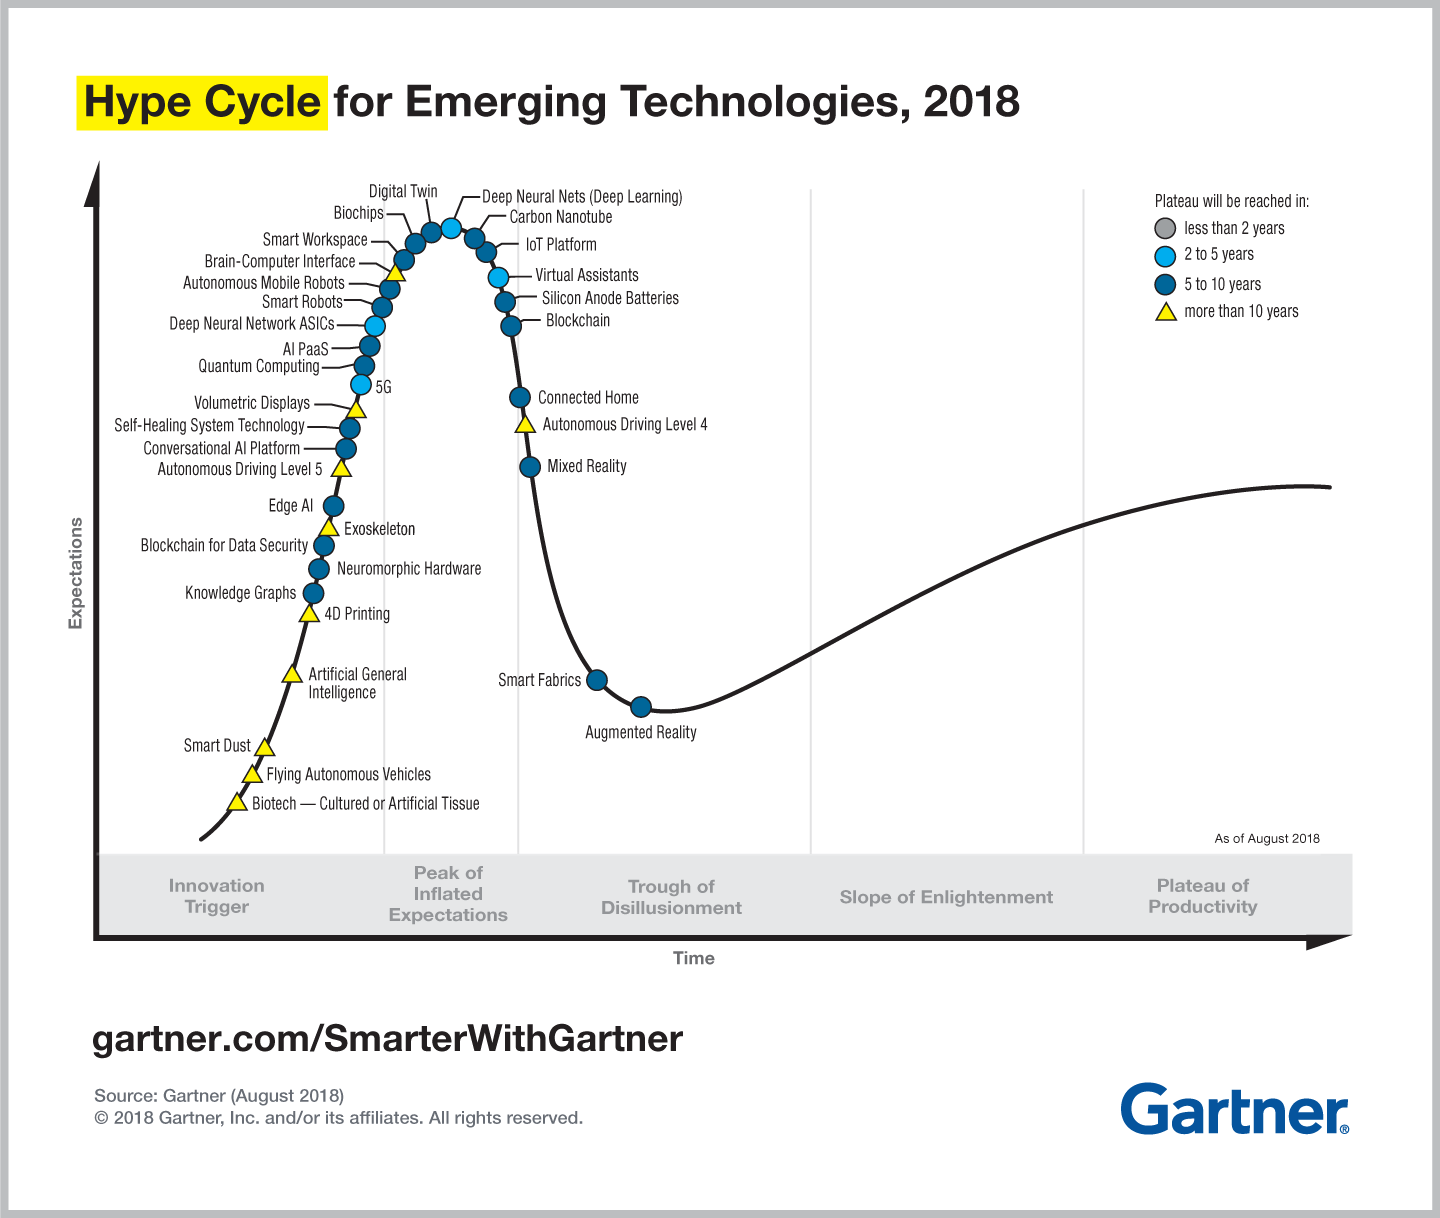
\includegraphics[width=1\textwidth]{PR_490866_5_Trends_in_the_Emerging_Tech_Hype_Cycle_2018_Hype_Cycle.png} 
                \caption{Gartner report of emerging technologies 2018}\label{gartner-2018}
            \end{figure}

            It is important to note though that as of 2018, it'll still take more than 10 years to reach a plateau of productivity.
            Although there is no mention about this technology in subsequent reports in the following year, two market revenue forecasts from 2015 until 2022 and 2018 until 2022 show a similar pattern in figure \ref*{statista-revenue}.

            \begin{figure}[h]
                \centering
                \subfloat[\centering \cite{Statista.24052021b}]{{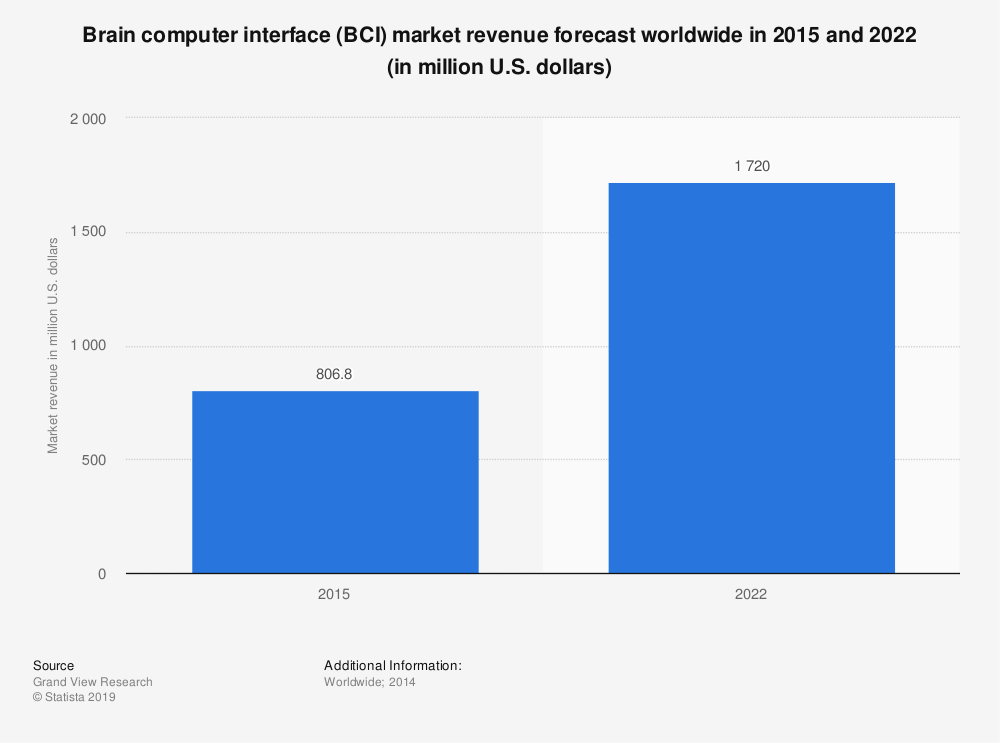
\includegraphics[width=0.49\textwidth]{statistic_id1015039_brain-computer-interface-market-value-worldwide-2015-and-2022.png} }}%
                %\qquad
                \subfloat[\centering \cite{Statista.24052021}]{{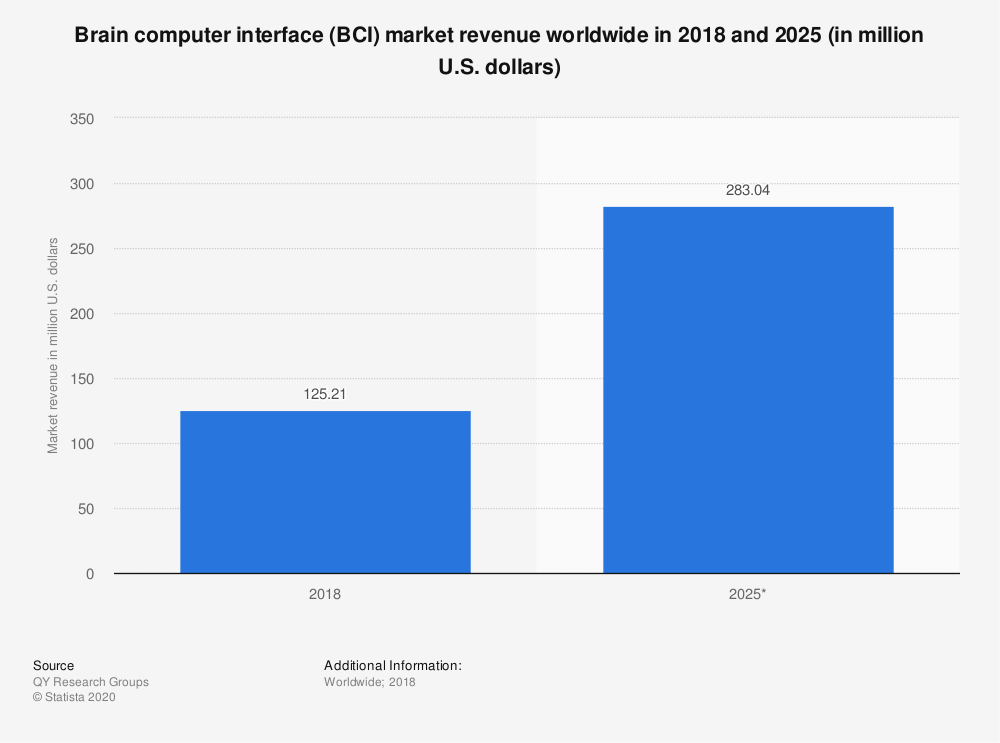
\includegraphics[width=0.49\textwidth]{statistic_id1015013_brain-computer-interface-market-value-worldwide-2018-and-2025.png}}}%
                \caption{Statista revenue forecast as of 2015 and 2018}%
                \label{statista-revenue}
            \end{figure}        

            Essentially the market revenue expectation has been very inflated from 2015 on so that it was corrected downwards in 2018. But although the absolutes growth was projected to only a small fraction, the relative growth potential stayed about the same of doubling within the next seven years. This is very indicative for the technology being overhyped, as Gartner explains: (\cite{Gartner.24052021})

            \medskip
                \emph{A wave of “buzz” builds and the expectations for this innovation rise above the current reality of its capabilities. In some cases, an investment bubble forms, as happened with the web and social media}
            \medskip

            Nevertheless, what this technology sets apart from other featured technologies is the fact that is has been around for a few decades and has been continuously researched upon. A strong indicator is the amount of organizations and conferences held about this entire discipline, as can be seen in section \ref*{related-work}. The fact that is has only been on the radar of early adopters and tech-enthusiasts in conjuction with market revenue projections is a strong indicator that this technology has reached a level of maturity which makes a widespread application outside of laboratories somewhat feasible.

            The latest \textit{2020 Gartner Hype Cycle} report shows already the enhanced version of bidirectional BCIs (titled \textit{"2-Way Brain Machine Interface"}) on the slope of innovation:

            \begin{figure}[h]     % h=here, t=top, b=bottom, p=page
                \centering
                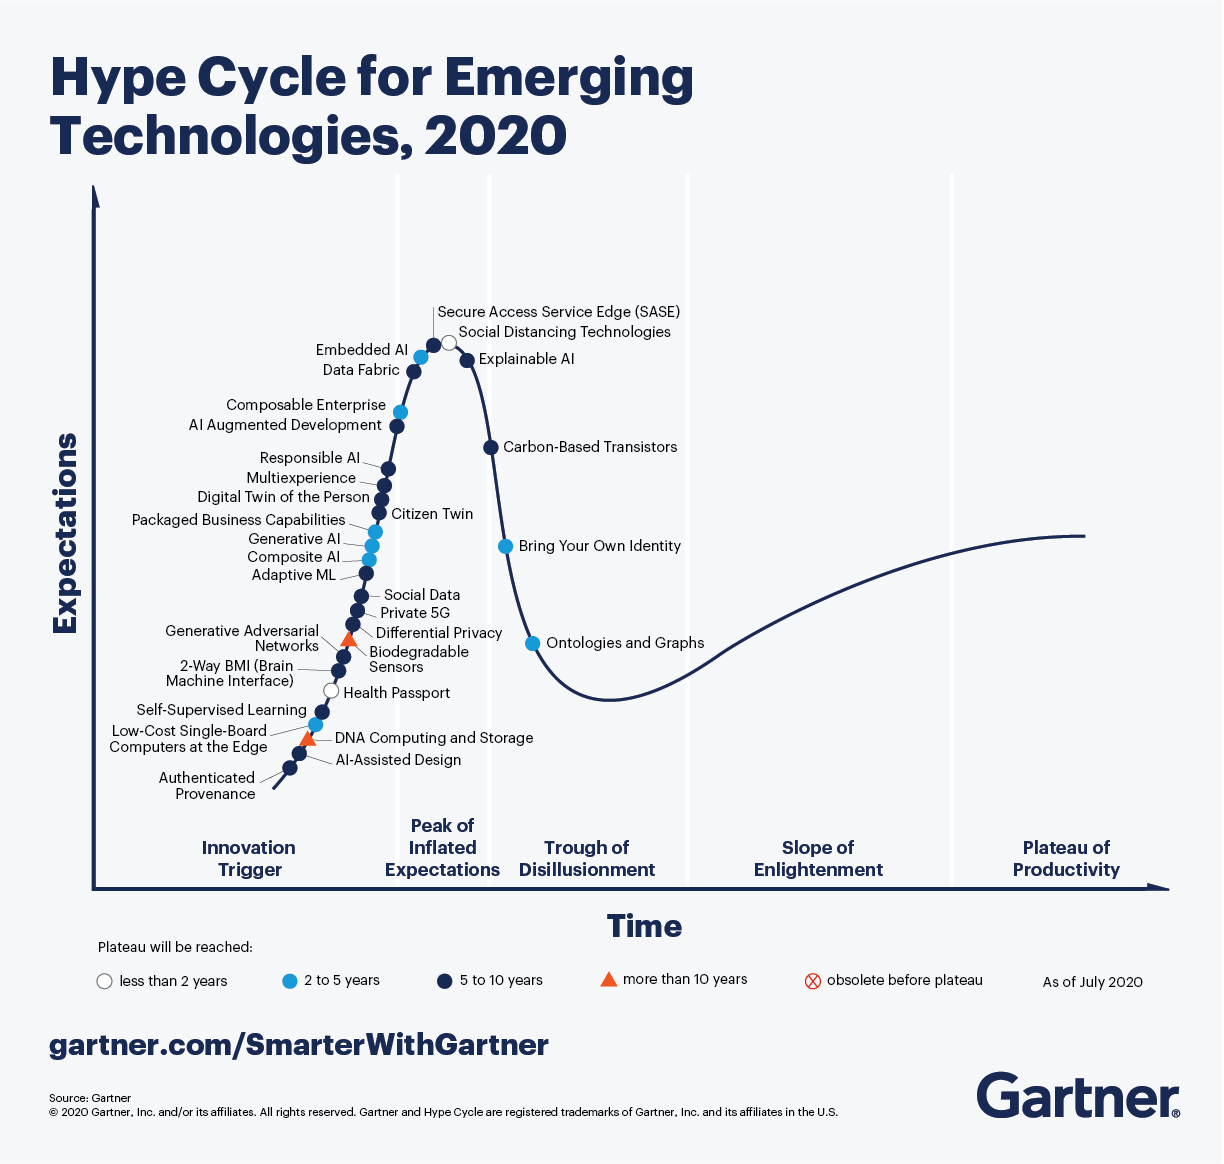
\includegraphics[width=1\textwidth]{gartner-hc-emerging-2020.png} 
                \caption{Gartner report of emerging technologies 2020}\label{gartner-2020}
            \end{figure}

            All in all, there are strong indicators that the technology gained traction over the last few years and could be considered a worthwhile investment if potential business cases are evaluated properly.

        \section{Brain-Computer-Interfaces}\label{intro-bci}

            In this section a general overview of the working principle of these interfaces will be provided. Since this study is aimed at computer science and HCI\footnote{Human Computer Interaction}, the neuroscience and medical domain will be only covered very briefly.

            First studies began by \cite{Vidal.1973}, who investigated the possibility to use EEG\footnote{Electroencephalogram} waves, which were first recorded by \cite{Berger.1929}, as a way to create a direct interaction between a machine and a human brain. 

            There are three types of BCIs: invasive, partially invasive and non-invasive. This depicts the degree of intrusion into the skull and brain tissue. \textit{Invasive} BCIs are electrodes, which are implanted directly into or onto the grey matter of the brain. This can cause long term issues like scars and also degraded singal strength according to \cite{Abdulkader.2015}. 
            Partially invasive BCI however are although located within the skull not in direct contact with the grey matter.
            Non-invasive BCI are only placed on the head without intrusion of any tissue.
            Due to the direct contact, invasive BCI provide the best resolution of the measured signals. Non-invasive BCI in comparison suffer from signal degradation and deformation of the cranial bone tissue. 
            Therefore partially invasive BCI are a compromise between good signal strength and the risk of medical conditions.
            Another potential advantage of non-invasive BCIs is that these Interfaces could be easier mass-produced and become affordable to consumers. Also they don't require specialized medical knowledge and equipment to operate.

            The way these interfaces work is based on the same principle: A human brain emits electrical signals, which can be picked up.
            According to \cite{Vidal.1973}, they can be described as follows:

            \medskip
            \emph{"Embedded in this sustained "spontaneous" or "ongoing" electrical activity, short, distinctive (0.5-2 sec) waveforms can be found that are evoked, for instance, when a brief sensory message (stimulus) such as a brief illumination of the visual field or a tap on the forearm is received by the subject."}
            \medskip

            Based on the origin within the brain, these can be correlated to certain stimuli, mental and emotional states (\cite{JardimGoncalves.2018}) and according to \cite{Waldert.2016} been used to drive \emph{an external effector or affecting internal body parts and functions.} The external effector is the use case which is being examined in this study.

            Without a BCI, interaction with a computer requires some physical interaction with devices such as keyboards, mouses, or gestures on a touch screen. There are mainly two different reasons, why these devices are a constraint to speed and efficiency of HCI. The first reason is a limitation on interaction speed: Although there is no definitive concensus about the speed of thinking, alone being able to type along the spoken word is unattainable for non-professional typists. A professional typist has to be able to type at 180 - 220 WPM\footnote{Words Per Minute} according to \cite{NCRA.25052021}. \cite{ScienceDaily.25052021} made a survey with 168.000 volunteers, where the fastest typists weren't even able to come close to this mark with 120 WPM. Therefore it is safe to assume that typing in the same speed as thinking is impossible except for rare individuals who devoted a significant time practicing. Secondly: in applications such as games, where reaction time and accuracy is the fundamental element for success or failure, an interaction based on motoric interaction with a physical pointing device has some significant drawbacks like limited accuracy, if the whole chain of wrist movement in conjunction with a mouse is under scrutiny. 

            If a BCI was to replace these types interaction, these constraints could potentially be alleviated and interaction based on physical interaction rendered obsolete. 

        \section{Working principle}\label{working-principle}         

            In order to understand the reasoning behind this study, the working principle of a BCI has to be established on a general level. Section \ref*{intro-bci} already established a high-level overview of different BCI technologies and how these are triggered by certain external stimuli. In this study only visual stimuli will be used and therfore explained in detail. The vendor, where the BCI in this study is from - \textit{NextMind} - does not disclose any details of the inner workings itself. However the interface works with flashing patterns, therefore it is safe to assume that the underlying technique used is the so called \textit{Steady State Visually Evoked Potential} - SSVEP in short. \cite{Sokol.1976} provides detailed inside into the topic from a neuroscientific point of view. The general principle is that any visual stimuli cause a certain pattern of waves within the visual cortex of the brain. These patterns are being evaluated by different means to assess if a certain pattern is being seen \textit{and} in focus of the person. 
            
            \begin{figure}[h]     % h=here, t=top, b=bottom, p=page
                \centering
                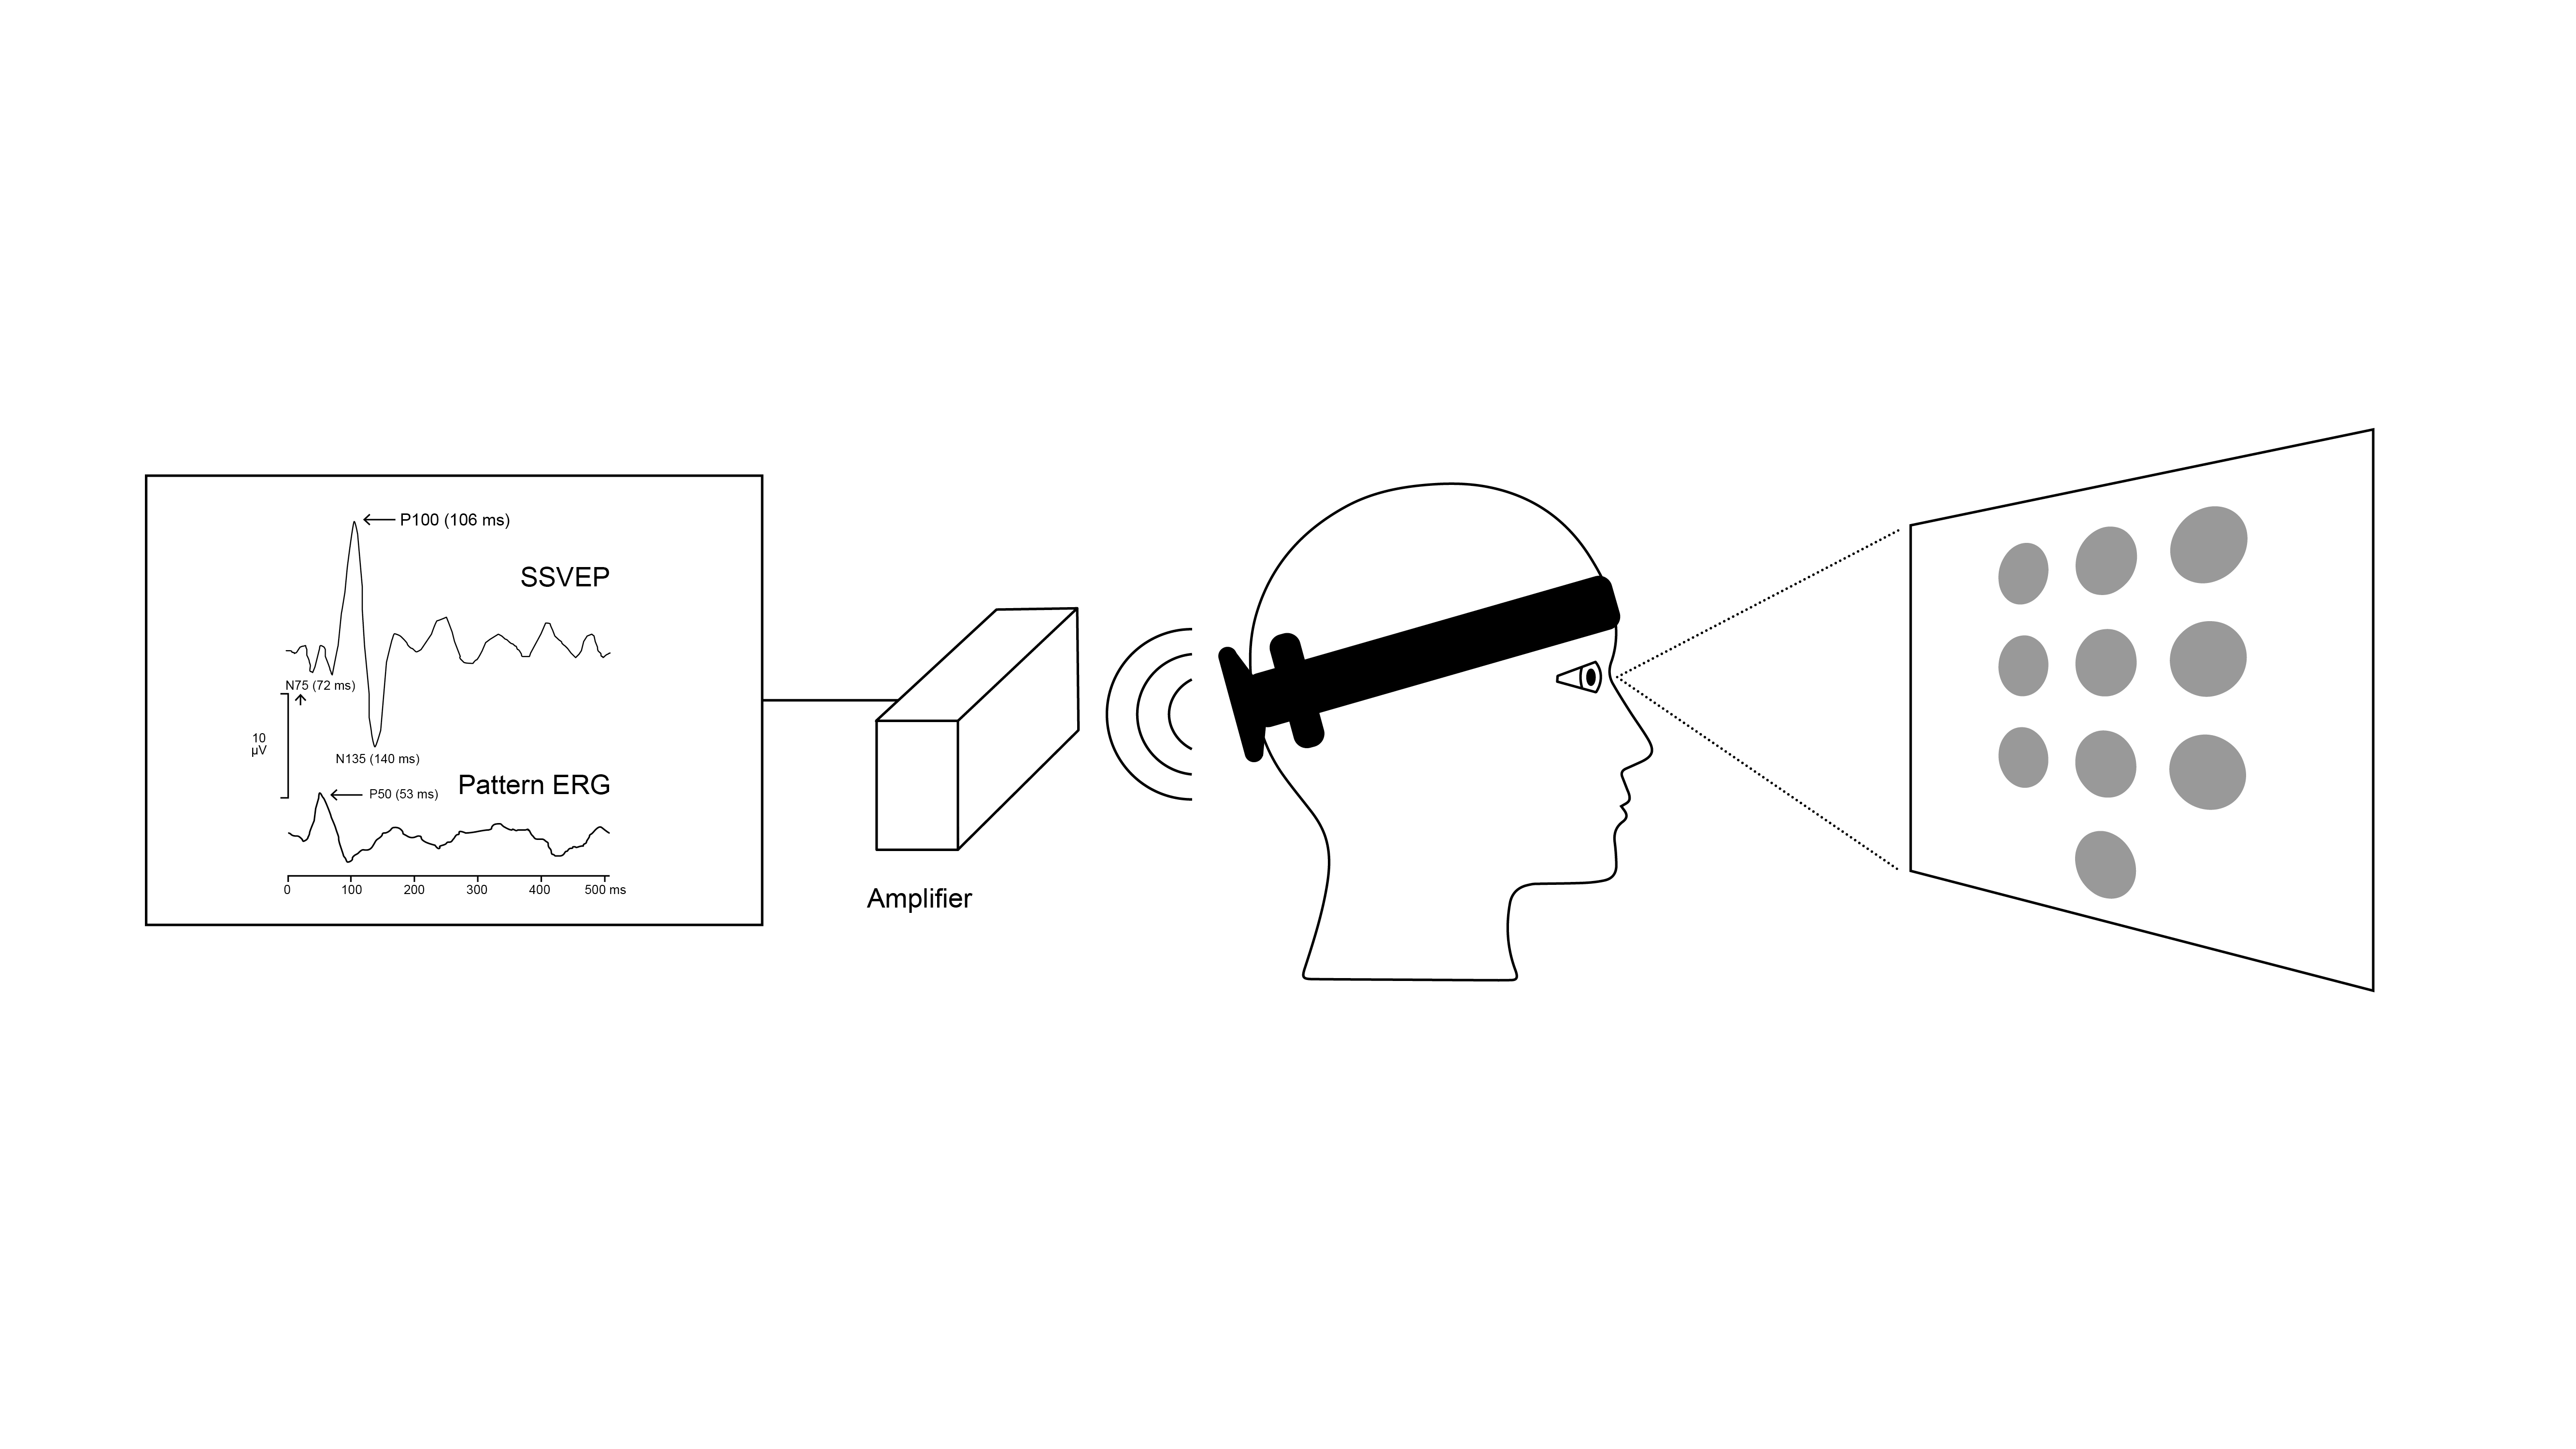
\includegraphics[width=1\textwidth]{Illu_Kopf2.jpg} 
                \caption{How VEP works in principle}\label{vep-principle}
            \end{figure}            
            
            According to \textit{NextMind} this is being done by feeding the sensor data through a trained neural network, which is able to return a confidence score for each target. The objects, which are being seen by the person, have been labeled \textit{neurotags} (\cite{NextMind.23112020}) from \textit{NextMind}. These neurotags can provide two different readouts: If it is triggered (i.E. \textit{seen}) and the confidence, which depicts the level of \textit{focus} of the user on the neurotag (\cite{NextMind.18112020}).
            
            \begin{figure}[h]     % h=here, t=top, b=bottom, p=page
                \centering
                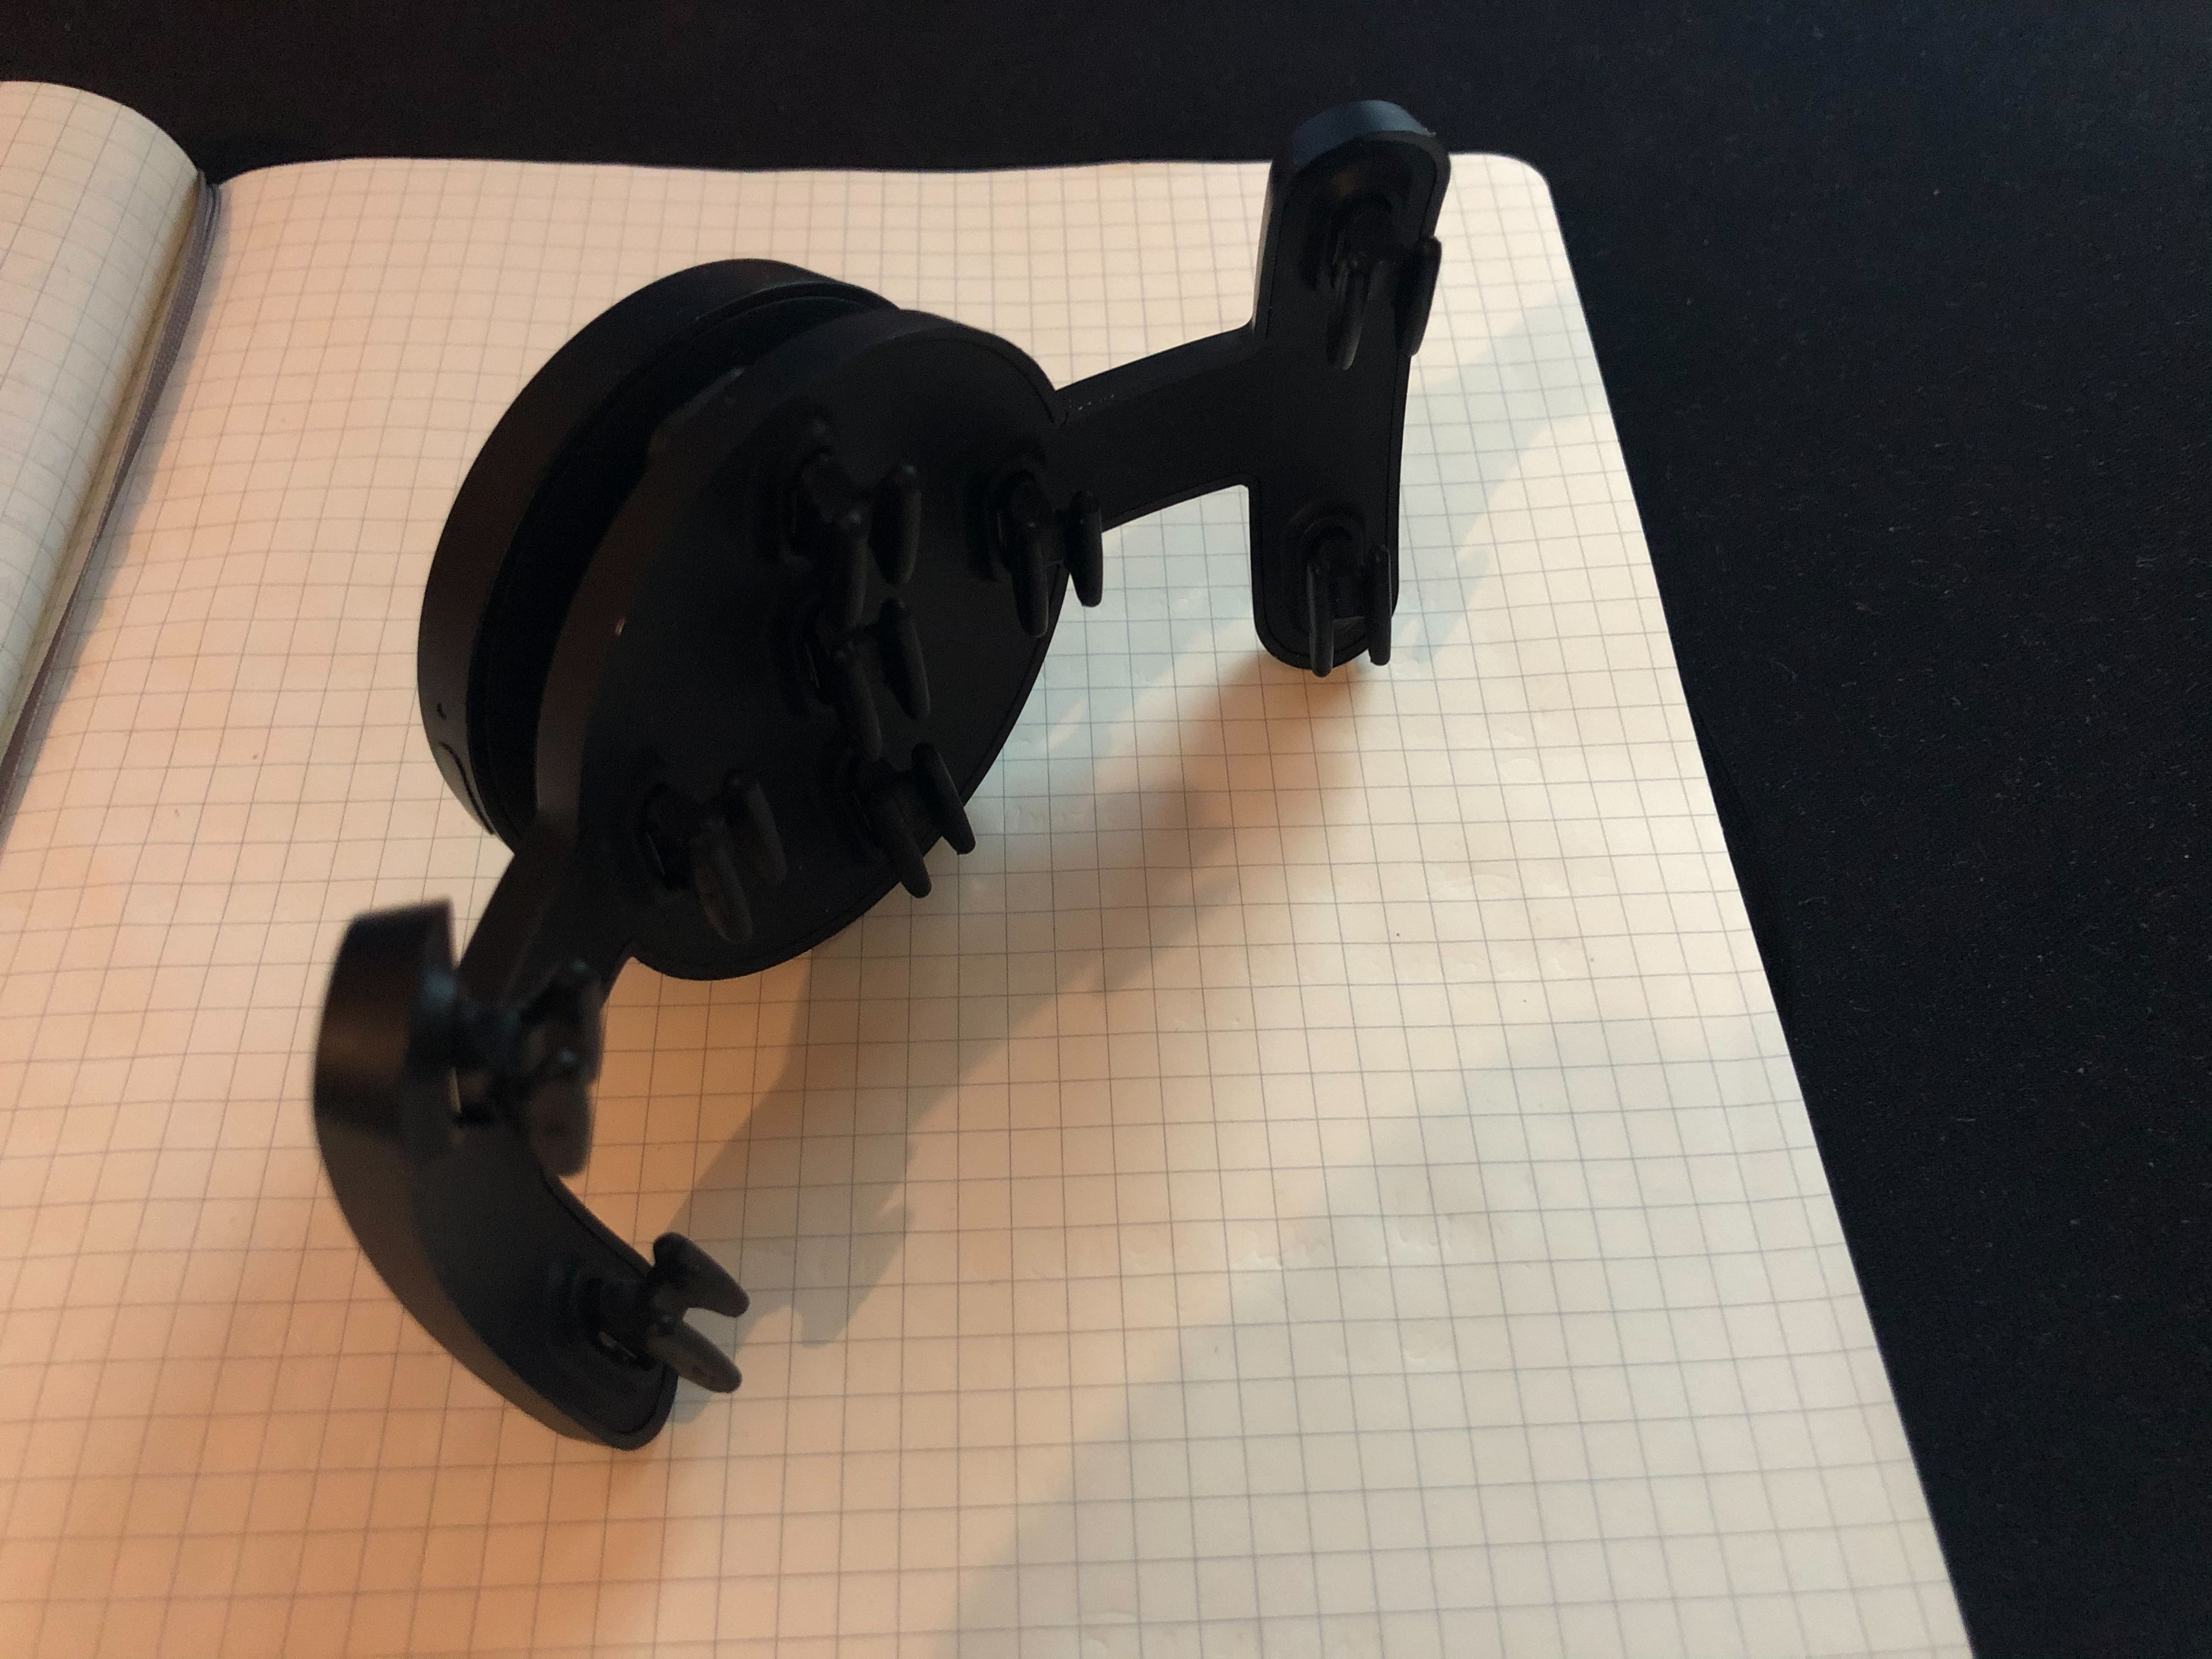
\includegraphics[width=1\textwidth]{electrodes-sensor} 
                \caption{Physical layout of the sensor}\label{electrodes-sensor}
            \end{figure}
            
            The physical layout of the sensor is shown at figure \ref*{electrodes-sensor}. It has 18 electrodes, which are arragend in pairs to cover the area, where the visual cortex is located, which is at the back of the cranium. These electrodes have a certain degree of freedom to their movement, which is beneficial since this mitigates the risk that small movements from the sensor alter the position of the sensor too much. It is battery driven and communicates via the Bluetooth Low Energy protocol. A headstrap keeps it in place.

        \section{Related work}\label{related-work}

            As previously mentioned in section \ref*{introduction}, research on BCIs is partitioned between four different domains: \textit{medical engineering, neuroscience, computer science, and HCI}. Apart from commercial entities such as \textit{Microsoft} or \textit{IBM} and scientific journals, the majority of the research community is clustered in three organizations: 

            \begin{itemize}
                \item ICBCI (\textit{International Conference of Brain Computer Interfaces}), which is a department of the WASET (\textit{World Academy of Science Engineering and Technology})
                \item EMBS (\textit{Engineering in Medicine and Biology Society}), which is a department of the IEEE
                \item BCI Society, which is an entity of its own
            \end{itemize}

            \medskip

            \emph{There are also research efforts in the east-asian region, according to corresponding tech-sites such as \cite{GlobalTimes.20042021} and \cite{TechwireAsia.24052021} but due to a language barrier, these sources cannot be considered.}

            \medskip

            To narrow the scope, where this research paper is located at, the considerations from section \ref*{use case-main} are taken into accout. As already established in section \ref*{working-principle}, the sensor used in this study uses SSVEP and is non-invasive in nature. Therefore the general scope of this research is located in the realm of \textit{non-invasive BCI based on SSVEP used for HCI}.

            \medskip

            \cite{Oralhan.2016} and \cite{Resalat.2011} investigated the effects of different twinkle frequencies and duty cycles on the efficiency on precision of SSVEP BCI. They found that a certain combination of these parametres on fact could improve the ITR\footnote{Information Transfer Rate}. \cite{Lee.2016} used a similar approach and found the ideal combination in conjuction with Korean characters.
            \cite{S.M.Abdullah.2014} used a consumer ready BCI by \textit{EMOTIV} to create a \textit{Matrix-Speller} in the Bengali language to allow people who have lost the ability to communicate to express themselves again. 
            \cite{Chen.2020} also used a SSVEP BCI to implement a BCI-speller and scrutinized the tradeoff between responsiveness and accuracy.
            \cite{Chen.2020} designed an interface which is operated by a SSVEP BCI to control a robot arm, which could administer food to disabled people.
            \cite{Soroush.2018} developed a SSVEP BCI which overcomes the necessity for training the sensor to the wearer. The prototype reached a similar precision as \textit{trained} interfaces.
            \cite{Gergondet.2015} investigated and selected certain visual stimuli which work best with certain use cases.
            \cite{Merino.2017} made a study, where participants controlled a UAV by using a SSVEP.
            \cite{Peters.2018} used simulated impairments to examine if usage of a SSVEP is still possible with medical conditions which affects speech and ocular impairments.

            Although not strictly within the SSVEP domain, the study by \cite{Beveridge.2017} showed very promising results by not using visual stimuli but mechanical ones, where he had teenagers playing a racing videogame with the aid of mechanical stimuli.

            There is a massive ongoing research effort to make the life of people who are suffering under ALS\footnote{Amyotrophic lateral sclerosis} better and improve their ability to communiate normally, by using SSVEP, a hybrid between an SSVEP and P300\footnote{An Event Related Potential (ERP) BCI}, or purely P300 based BCI. A significant number of relevant studies has been published in the BCI Society Journal: \cite{Sugata.2016}, \cite{Holz.2015}, \cite{Speier.2017}, \cite{Geronimo.2017}, \cite{Speier.2018}, \cite{Mowla.2017}, \cite{Huggins.2016}. All these studies aimed to provide a better understanding and performance of using BCI on people with medical conditions, which cause serious physical impairments.

        \section{Establishing a use case}\label{use case-main}

            Establishing a use case in the context of this study is a pivotal point hence this section will be split up into several sections: 

            \begin{enumerate}
                \item General considerations
                \item Deduction of the core points of this study
                \item Evaluating the constraints of a participatory study
                \item Deduction of use case
                \item Conclusion into hypothesis and use case
            \end{enumerate}

            \subsection{General considerations}\label{general-considerations}

                The first step in conceiving any potential way of using such a device is to evaluate the way any user could interact with a BCI with a computer. According to \cite[4.13]{Buxton.2010} the way users interact with a device require an agent of control i.e. a hand, what is being sensed by the device (position, motion, or pressure) and the number of dimensions being sensed (1, 2, 3). This results in a different input taxonomy for any given device. However, a BCI does not have either of these parametres, since the interaction does not require physical interaction. Hence a classification by means of using a taxonomy cannot be achieved. Where the interactions of BCIs can be compared to those classified by taxonomies is the way their functions result  in actions or events towards a user interface.

                The API\footnote{Application Programming Interface} endpoints of the NextMind sensor offers two different modes of interaction. These are explained in the SDK\footnote{Software Development Kit} of the sensor in detail: \cite{NextMind.18112020}.
                They are depicted as \textit{tracking results} with a \textit{hit} property and a \textit{confidence} metric. A \textit{hit} is a two state interaction: the neurotag is being seen by the user and subsequently recognized by the sensor and its backend or it is not. The confidence property depicts the attention which the user is paying to the \textit{neurotag}. This is a continuous decimal value between 0 and 1.
                The fact that these types of interaction are based on neural activity raises the question if a pure mapping of continuous and discrete input modalities to established interfaces would be beneficial to the user experience. Under the reasonable assumption that without any training the metric \textit{focus} can only be deliberately controlled on a very coarse level, the necessary sensitiviness required for modern GUIs\footnote{Graphical User Interface} can not be achieved with this particular sensor. The remaining two state property, which can be utilized to select or deselect certain objects also only allows for limited interaction. However, these neurotags can be placed in arbitrary places. Although a \textit{toggle}-like behavior is not mentioned explicitly, it might be possible to de-select any activated neurotag when the \textit{focus} property falls under a certain value.

            \subsection{Corepoints of this study}\label{corepoints}

                Based on the previous reasoning, the following questions can be raised in regard to the feasibility of any interface which could potententially be conceived with this technology:

                \begin{enumerate}
                    \item How fast is the perceived and measured reaction time of these neurotags?
                    \item What is the minimum size the neurotags have to have in order to be recognizable?
                    \item Is the interface usable for brains of all ages or do gerontological effects have an effect on usability?
                    \item Do certain medical conditions (i.e. attentiveness disorder) have an impact on the usability?
                    \item How fast can a user switch between neurotags?
                    \item Is a BCI controlled GUI intuitive to use?
                    \item Does a personal affinity to technology have an influence on the perceived difficulty of interaction?
                \end{enumerate}

                These questions can be clustered into two groups: \textit{neurological} and \textit{interaction}. But all these considerations open up a vast space of potential cases, hence the priority is to examine whether these interfaces are generally usable by the majority of users and if these interfaces are intuitive to use. Out of this list only the points 1, 2, 3, 5, 6 and 7 can be applied to a general audience. Considered the possible interactions with the \textit{NextMind} sensor, a study which focuses on the neurological domain makes more sense in the context. This leaves the points 3 and 5. Although these are two different topics, the setup of the experiment itself will show that in fact number 5 is actually the driving metric to answer this question, which will be discussed in section \ref*{survey-framework}.

            \subsection{Constraints of a participatory study}
            
                Although this study won't use the framework of an \textit{AttrakDiff} survey, which was designed by          
                \cite{Hassenzahl.30092020}, it is still worth considering how a potential use case might perform in the context of an \textit{AttrakDiff}. The reasoning is that a survey, which is entirely constructed to serve the purpose of producing results in favour of the study, might be harder to grasp for the participants in the experiment. The reason being that an interaction purely for the sake of interacting with something does not provide an incentive for the user to do so. As a consequence, the results which are produced by the participants, might be skewed due to a lacking frame of reference.

                \begin{figure}[h]     % h=here, t=top, b=bottom, p=page
                    \centering
                    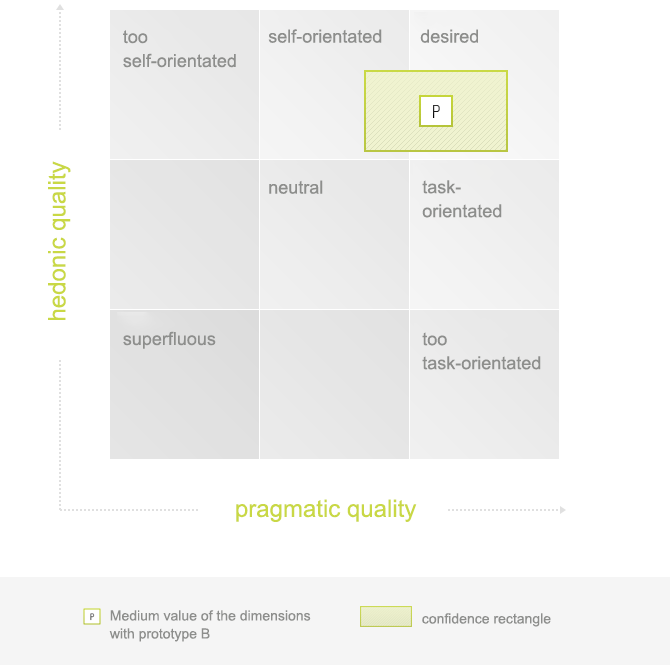
\includegraphics[width=1\textwidth]{einzelauswertung_en.png} 
                    \caption{AttrakDiff results for a given interaction model, Source: \cite{Hassenzahl.30092020}}\label{AttrakDiff}
                \end{figure}

                Figure \ref*{AttrakDiff} shows two axes which depict the hedonistic quality of an interaction, which is a metric of pleasure and the pragmatic quality which depicts a metric of \textit{ease of use} or \textit{technical quality}. Even without any deeper knowledge it is safe to assume that it is preferential for the interaction to be located in the upper right corner, since this makes it \textit{"desireable"} instead of \textit{"unnesessary"}. Given that, it is certain that any interaction needs a way to facilitate pleasure in the user.

            \subsection{Deduction of use case}\label{use case}

                Concluding the two parametres \textit{frame of reference} and \textit{facilitation of pleasure} into a coherent picture, it can be inferred that the experiment has to be set up in way that gives the participants a familiar use case which facilitates positive feedback. 

                As already established, this study will examine gerontological effects in the context of an interaction. Therefore the age of participants will very likely vary to a wide degree, what necessitates a use case which is common to all age groups alike. Because people above a certain age did not grow up with computers, an experiment which relies heavily on the usage of computer as main point of interaction is very likely not a good choice due to the difference in proficiency. One example where both these criteria are met is a remote control for a television. Although nowadays there are computers involved, the interaction hasn't really changed in the last decades on a general level.

                Nevertheless the working principle of the BCI is a visible flashing pattern, as established in section \ref*{working-principle}. Therefore the representation of some kind of GUI on a display is still necessary. Since VR goggles provide better isolation from external visual stimuli, the representation within a VR application was chosen. 

                \medskip

            \subsection{Concluding hypothesis and use case}\label{hypothesis}
            
                Section \ref*{corepoints} established that age is the first parameter to examine in this context, therefore the fundamental research hypothesis can be defined as follows:

                \medskip
                \emph{"Age does not have a detrimental effect on the ability to use a non-invasive BCI based on VEP technology."}
                \medskip

                In Section \ref*{use case} the fundamental reasoning behind the use case, which provides the necessary framework for this study was established:

                \medskip
                \emph{A GUI which represents a tv remote control will be presented to the participants within a VR environment.}
                \medskip

        \section{Beyond the scope}\label{beyond}

            The case in this study is fairly limited in the realm of BCI. Section \ref*{related-work} already briefly mentioned that the general research on BCI has several fascinating topics to explore. This section aims to broaden the horizon on the realm of BCI technology.

            \paragraph{Picture synthesis}

                In 2019 \cite{Rashkov.2019} published a paper which outlined the reconstruction of images seen by individuals by means of a BCI. They used a 128-channel EEG cap to record brainactivity in a 1...35Hz bandwidth while being shown videos of different subjects. The signals were treated with a PCA\footnote{Principal Component Analysis} to create a 20-dimensional feature vector which is feeded into a classification model, which yields the results:

                \begin{figure}[h]     % h=here, t=top, b=bottom, p=page
                    \centering
                    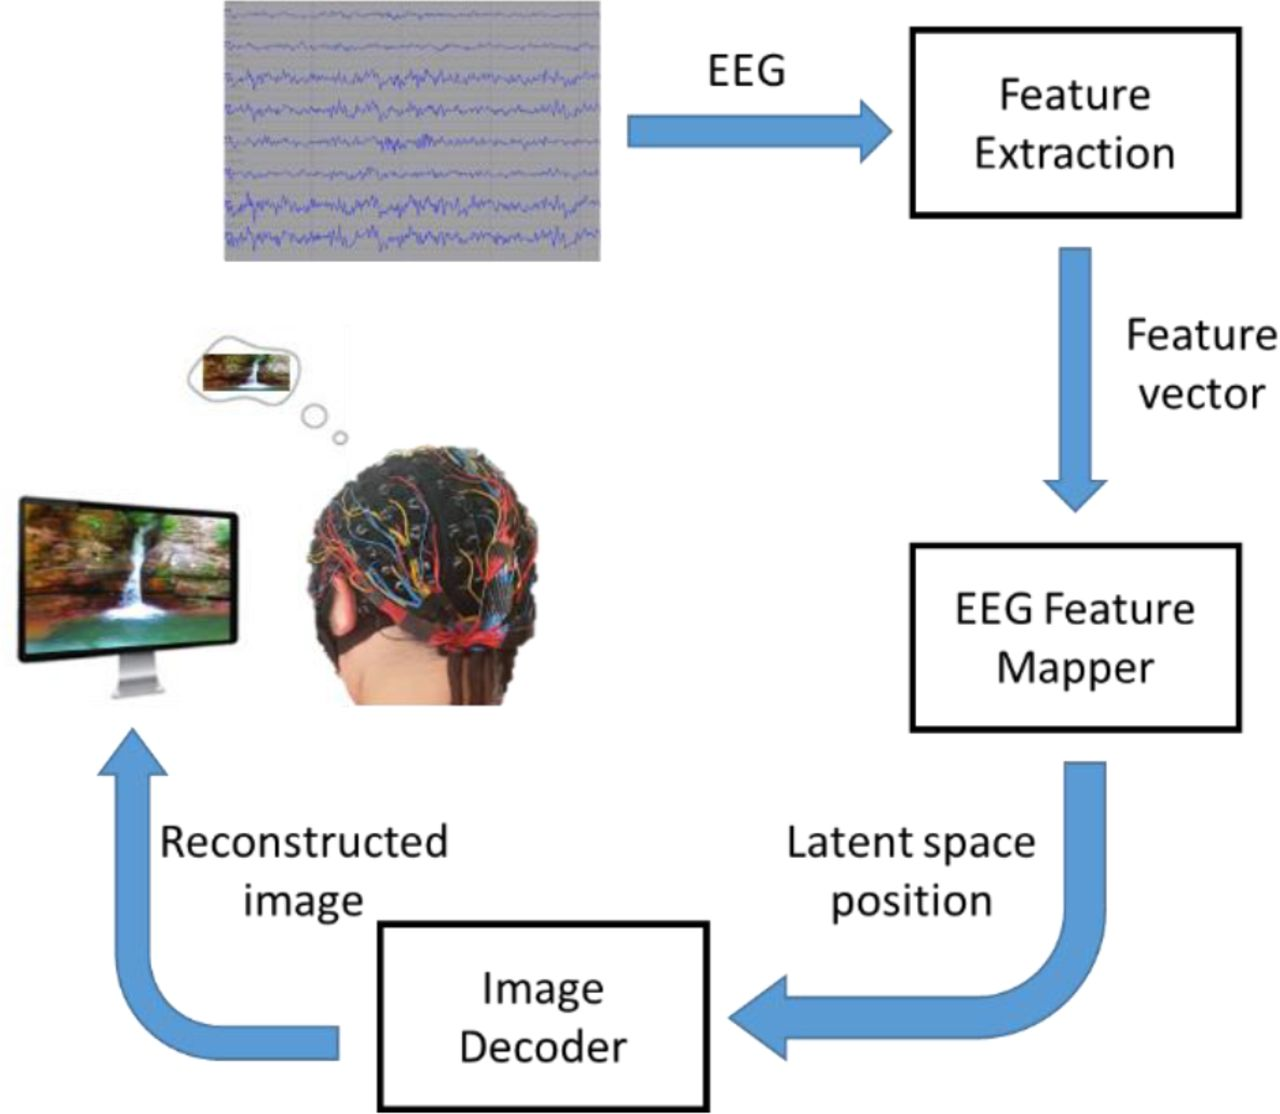
\includegraphics[width=1\textwidth]{F2.large.jpg} 
                    \caption{General scheme of neurofeedback model, Source: \cite{Rashkov.2019}}\label{image-synthesis}
                \end{figure}

                \cite{Oneill.14112019} wrote a good summarized article about the paper alongside results and a video which features a demonstration. On the other hand \cite{HernandezCarmona.2019} used a similar approach to enhance grasping of robotic arms by means of deciding on the correct technique to grasp based on image reconstruction from a BCI.

            \paragraph{Controlling vessels, aircraft and spacecraft}
                
                Since BCI like the P300 have been used as neuroprosthetics for physically impaired people, there are efforts made to study a broader application of BCI to control machines or vessels. \cite[]{Choi.2018} published a study, where invasive BCIs for direct control of machines were examined. They came to the conclusion that this is very much possible but requires several advancements to gain really high quality data for fine-motoric movements. This also requires that electrodes have to be implanted deep inside the brain in order to gain high resolution results.

                \cite[]{WilliamKucinski.2018} published and article on the SAE News homepage, describing a report published by the DARPA where an individual was able to control three warplanes in a simulator. The novelty in this research was also the feedback given to the individual, thereby posing a bidirectional BCI. As of Q2 2021, this article is no longer available on the DARPA homepage but several other news organizations wrote about this: \cite[]{Stockton.03052015}, \cite[]{Blair.2018} and \cite[]{Tucker.09062018}. Since the DARPA is well-known in their field for pioneering the research, it is very well feasible outlook to have BCIs in the future, which allows for control of not only aircraft but also ships and spacecraft.

            \paragraph{Improving human learning rate and augmenting system performance}

                In an article published by the Journal of neuroscience methods by \cite[]{Miranda.2015} the efforts by the DARPA\footnote{Defense Advanced Research Projects Agency}, which is a US federal agency to advance technology for defensive efforts, were outlined. These grouped into prosthetics and rehabilitation as well as efforts to improve human training and performance. The latter has fascinating research on Improving the learning rate of the human brain:

                \medskip
                \emph{The Narrative Networks (N2) program is developing new techniques to quantify the effect of narratives on human cognition and behavior, including initial development of a closed-loop BCI system that adapts a narrative in response to a listener's EEG signals. Such a system would have numerous applications to training and human performance domains.}\cite[]{Miranda.2015}
                \medskip

                Further applications were the integration of a \textit{Human-in-the-loop}, scenario, where intelligence analysis and threat warning. A 10-fold improvement in analysis throughput was achieved in the former case. In the latter case of threat detection the incorporation of a BCI-enabled human increased the probability of threat detection to 91\% compared to 53\% detection rate solely relying on computer vision.

            \paragraph{Transferring thoughts over the internet}

                A paper published by \cite[]{Martins.2019} outlined the possibility of using nanotechnology to insert sensors to every single neuron and synapse in the human brain to have a real time stream from the within the human brain with a resolution down to a single neuron. This would allow for every human having a digital twin of himself in the cloud, having access to the whole repository of human knowledge withoug timedelay and even share experiences, thoughts and memories with other people.

                \begin{figure}[h]     % h=here, t=top, b=bottom, p=page
                    \centering
                    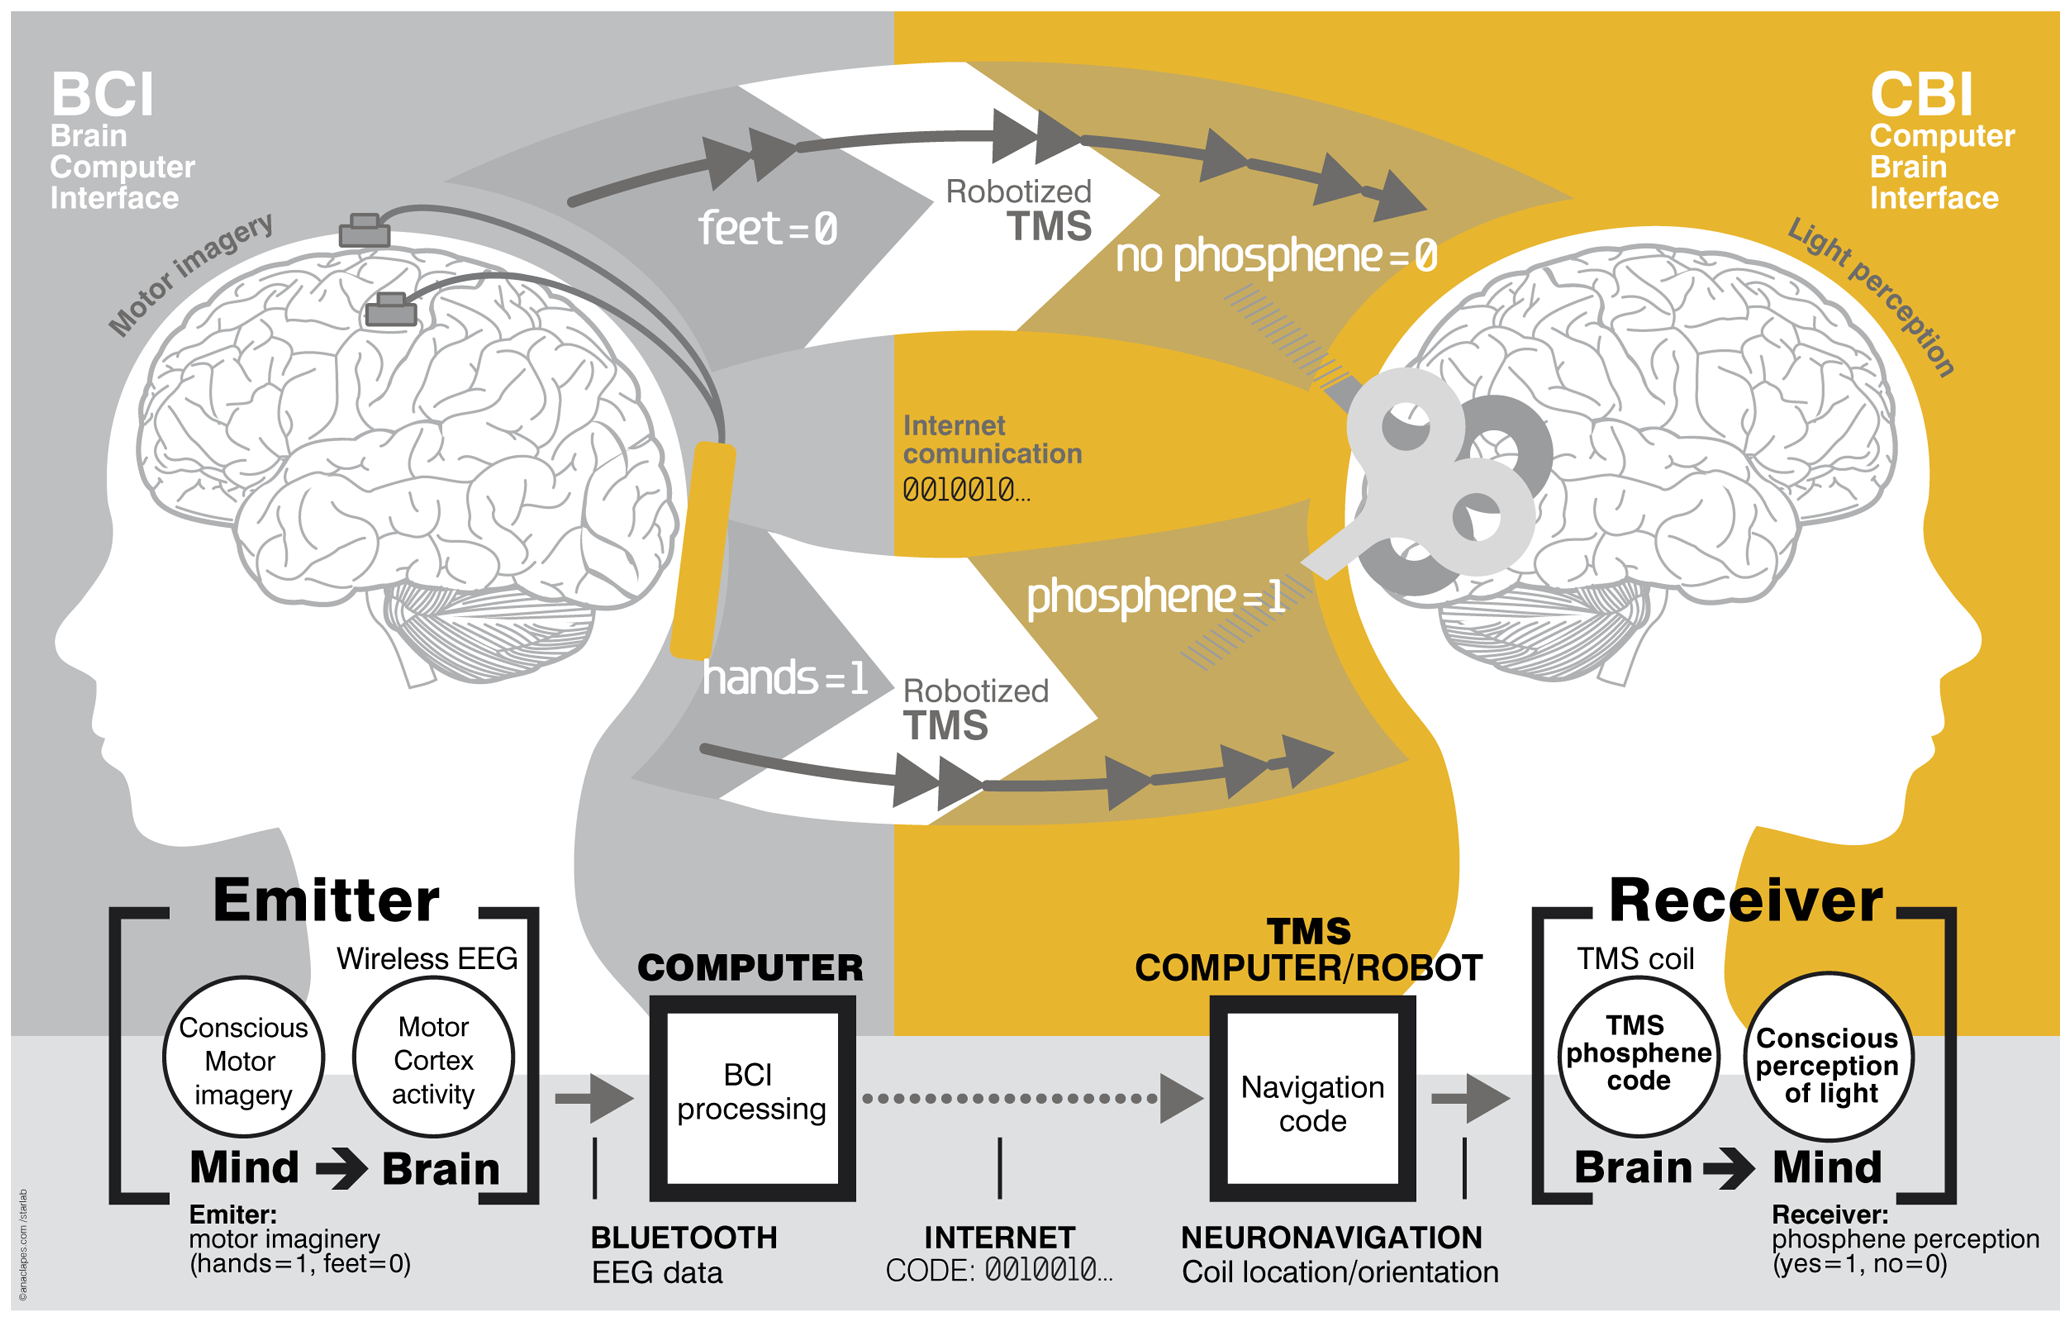
\includegraphics[width=1\textwidth]{pone.0105225.g001.PNG_L.png} 
                    \caption{B2B communication signal chain, Source: \cite{Grau.2014}}\label{b2b-chain}
                \end{figure}    

                A little less futuristic is a study published by ABC News: \cite[]{Lee.2016} outlined in figure \ref*{b2b-chain}. In this case for the first time in human history, conscious communication from one brain to the other without the involvement of sensory or motoric stimuli was achieved. This is called a B2B or Brain-to-Brain communication. The according paper was written by \cite[]{Grau.2014}. In this case two humans exchanged the greetings \textit{Hola} and \textit{Ciao} over the internet from India to France.

            \paragraph{Data privacy}

                With the latest innovation in the field of BCI and BMI a new concern arises along with them: privacy. \cite[]{Greenberg.2019} published a paper, where she outlined the current status and outlook on data privacy in regard to brain data, where the juristictions of the EU, United States and Canda were compared with their different approaches:

                \medskip
                \emph{In relation to the governance of personal data in the private sector, the United States adopts a self-regulatory mechanism, while the European Union assumes a rights-based approach, with Canada's position being intermediate to the two extremes.}, \cite{Greenberg.2019}
                \medskip

                She concludes that \emph{As BMIs enter the marketplace, legal and ethical questions pertaining to brain data privacy are certain to arise}\cite[43]{Greenberg.2019} and makes policy recommendations to be implented in order to guarantee privacy. These recommendations outline a \textit{privacy by design}, improvement of transparency and general sharpening of existing policies to better suit the requirements of brain data applications.

        \section{EEG acquisition devices}

            Concluding section \ref*{intro-bci} and \ref*{beyond}, it is reasonable to talk about some technical implications of BCIs and their limitations. In technical terms, these are EEG acquisition devices from the medical domain and only gather EEG brainwaves from certain regions of the brain. The placement of the electrodes on the skull determines which domain of brain activity will be recorded. 

            There is a great variety of these different EEG acquisition devices on the market. Ranging from consumer-grade cheaply and readily available sensors which cost a few hundred euros up to medical grade devices. According to \cite{Zerafa.2018} the difference in price and quality are mainly determined by the factors amplifiers, electrode type and count, and transmission technique, which could be wired or wireless.

            Since these sensors measure electrical potentials, the actual resolution of the electrodes and amplifiers is the single most influental parameter governing quality. \cite{Zerafa.2018} used the SNR\footnote{Signal to Noise Ratio} of different sensors to compare them to one another, because quality in electrical measurements is best compared using the SNR value of each measurement:

            \begin{figure}[h]     % h=here, t=top, b=bottom, p=page
                \centering
                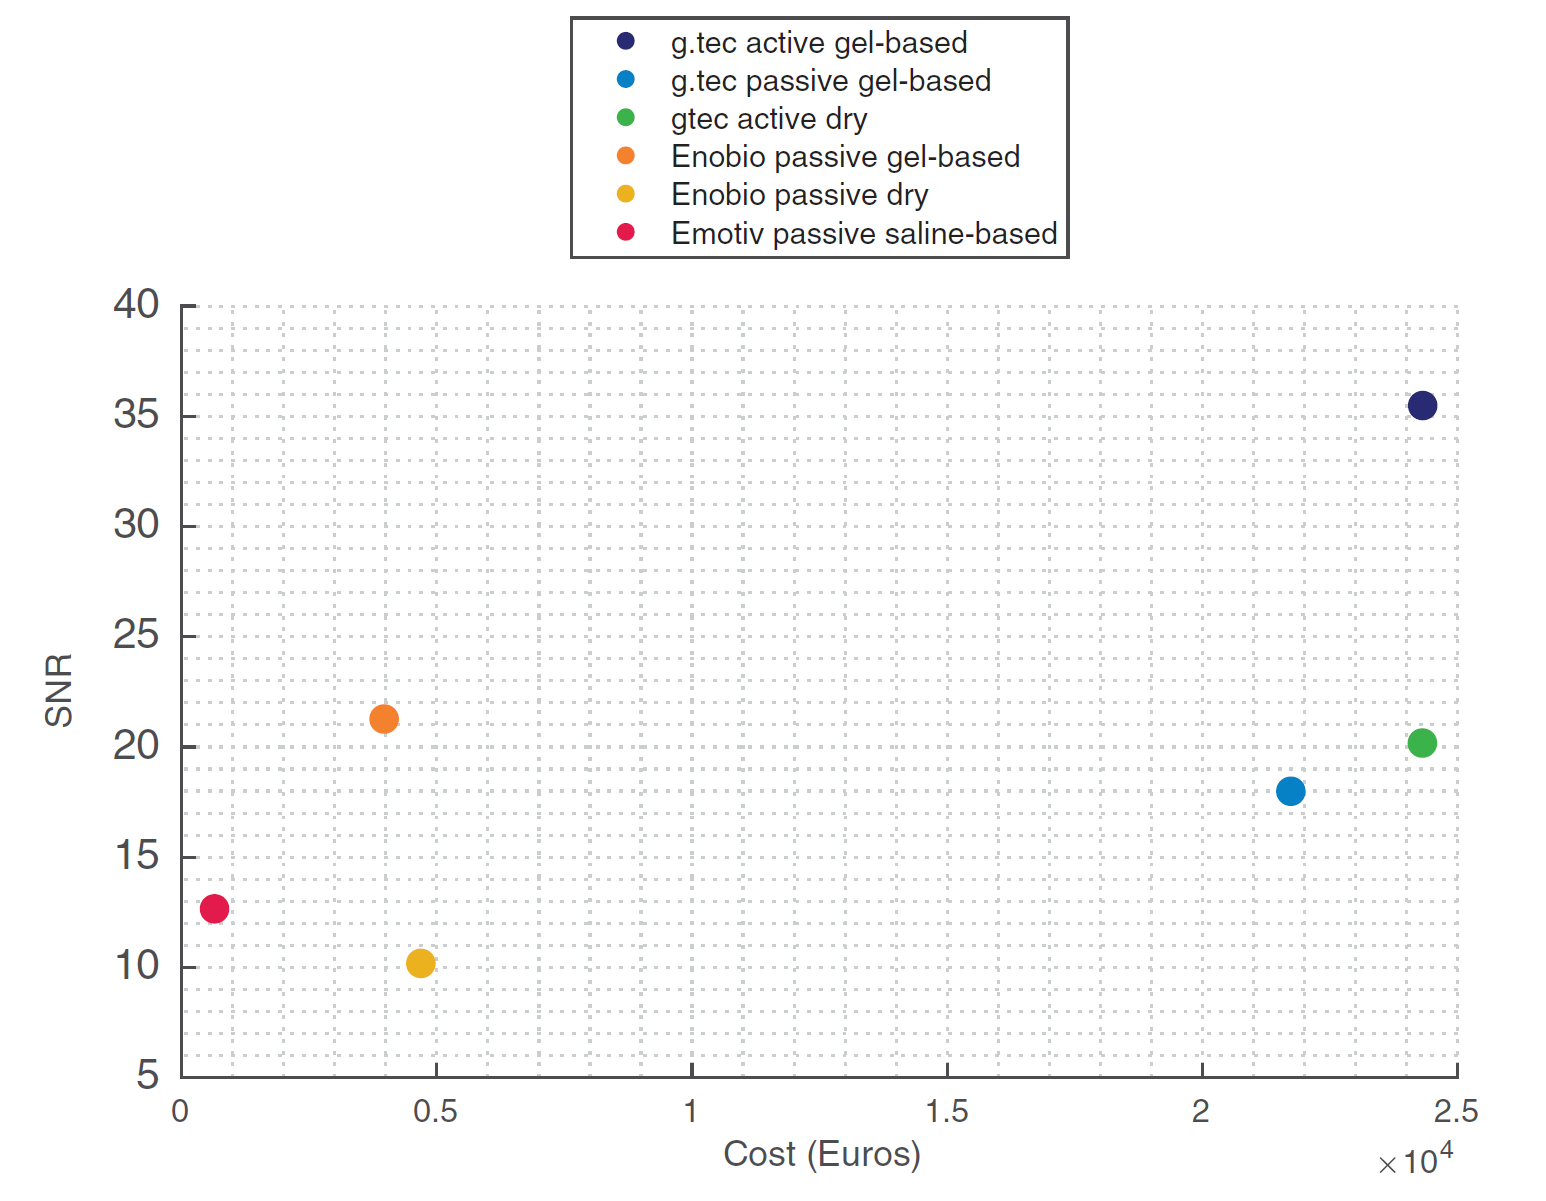
\includegraphics[width=1\textwidth]{eur-vs-snr.PNG} 
                \caption{SNR plotted against price, Source: \cite{Zerafa.2018}}\label{snr-eur}
            \end{figure}              
                
            Figure \ref{snr-eur} shows the picture that \textit{cheaper} sensors tend to have a worse SNR than more expensive ones with one exception which performed better. However, the cheaper sensors were perceived more comfortable and their set-up time was significantly less compared to fully fledged medical devices, which made them the better choice for experimenting and rapid prototyping. Also the expensive sensors required special treatment with gels and saline solutions, which wasn't necessary on the dry-electrode setup of the cheaper sensors. The conclusion of \cite{Zerafa.2018} was that either of those two caterogories have their advantages in their own domain and there is no \textit{best choice}.

    \chapter{Study Framework}\label{survey-framework}

        Based on section \ref*{hypothesis} the study, which investigates whether the hypothesis holds true or not has to be defined in a theoretical way. This is being done by answering four seperate questions in this context:

        \begin{enumerate}
            \item The general scope of this study
            \item Considerations for the questionnaire
            \item Statistical significance
            \item Time vs age correlation
        \end{enumerate}

        \section{Scope of the study}\label{study-scope}

            The first apsect which defines the general layout of a study is determined by its scope. Apart from domain specific studies like for example clinical trials, there are two general types of studies: \textit{qualitative} and \textit{quantitative} ones. The former one depicts a study where the number of conducted experiments are in the range of one or lower two digit numbers like 20-30, which is common according to \cite[302]{Doring.2016}. Quantitative studies often have four to five digit numbers of testcases according to \cite[305]{Doring.2016}. The latter ones are far more resource intensive however than their qualitative counterpart. A subset of qualitative studies are explorative studies. In these studies there have not been any previous research efforts so they're often considered preliminary to evaluate the scope and nature of the problem. Since all of these studies have a different objective target, the requirements regarding the samples are different in order to mitigate the risks of a previously unknown factor to skew the results. This might result in rendering a complete quantitative study irrelevant due to previously undetected errors. For this reason \textit{quantitative} studies have to make careful deliberation about the characteristics of the participants in order to avoid a systematical error. This is often done by using \textit{Qualitative} studies which are taking a different approach in regards to sampling the population. Since the number of participants is fairly low, they are often hand selected to pick certain characteristics deliberately. For the scope of this study, these deliberations are discussed in section \ref*{considerations}. 

            Regarding the scope of this study, two main questions have to be answered, to evaluate whether a quantitative, qualitative or even exploratory study is the best approach:

            \begin{itemize}
                \item Is there a previous study, which already established key-findings to build upon?
                \item How many resources are available to conduct the study?
            \end{itemize}

            To answer the first question regarding previous studies to build upon, none of the studies discussed in section \ref*{related-work} had the age as a core point. Nor were there any conclusions drawn from a study, which found that age had a significant impact on the results. Age did always play a major role, because BCI are often used as neuroprosthetics, whose usage is being found more often among the older population. More so the \textit{NextMind} BCI has not been subject of a scientific study at the time this study has been written.

            In regards to the second question, is has to be taken into account that the amount of people involved in this study is very limited and there was no additional funding granted to help with procuring more resources. All preparations and the experiment are being done by a single person, which severly limits effects of scale to sample a larger population.

            When these two facts are taken into account, the clear picture of a qualitative study can be drawn. More so, it is reasonable to design this study in an explorative way such that it can be determined, if there is evidence which supports a quantitative study in order to determine exact resons why the hypothesis might or might not hold true.       

        \section{Questionnaire Considerations}\label{considerations}

            The primary goal of the survey is to find empirical evidence that age does not affect the ability to use a BCI. In order to exclude certain parametres, which might cause an unwanted effect, potential disturbance parametres have to be identified and discussed:

            \begin{itemize}
                \item Age
                \item Gender
                \item Quality of the sensor readings
                \item User wears glasses
                \item Cognitive impairments
                \item Medication or drugs known to affect EEG readings
            \end{itemize}

            Furthermore participants of the study should disclose if they had previous or ongoing conditions of seizures or epilepsy, especially in case of light or flashing related cases since the visual cues in the experiment might trigger a medical condition.

            Apart from the demographic parametres of age and gender, the other factors have to be considered to prevent potential malformed data. Firstly, a condition which causes a detrimental effect on the ability to see and identify patterns such as deteriorated eyesight might have a dampening effect on the ability of the visual cortex to create the required brain waves, if the person can't see clearly. However, since the setup of the experiment allows for glasses to be worn, this will not be considered a concern. 
            Medical conditions or drug intake might also have a huge impact on the results. Diseases such as dementia or alzheimers or drug intake such as alcohol or caffeine have to be considered in the individual performance of each subject. \cite{Kenemans.1995} showed that caffeine intake has an effect on brain wave activity, therefore this has to be taken into account.
            Lastly the readings of the sensor will very likely be different for each experiment. Since the sensor provides quality readings, these will be considered in the data evaluation. Nevertheless, there will be a questionnaire provided which will ask the user after experiment if he experienced any of these effects to have a possible explanation for potential outliers.

            \medskip

            This study also assumes that gender has no effect on the study, because the brain of men and women is at least structurally identical. Therefore age is the only parameter which is the variable in this study.

        \section{Statistical significance}\label{doe}

            Plots of data can be misleading in terms of accuracy or results regardless of how well the data was preprocessed. For this reason, is has to be proven that the collected data actually proves a statistical significance in regards to the corresponding hypothesis. This section operationalizes the hypothesis such that it becomes evaluable.

            \medskip

            The hypothesis states that \textit{Age does not have a detrimental effect on the ability to use a non-invasive BCI based on VEPtechnology} - see section \ref{hypothesis}. The question is how to measure if an effect is present or not. The usual method in all kinds of studies of qualitative or quantitative type is to disprove the so called \textit{null hypothesis} - $H_{0}$. The part of the hypothesis about \textit{[...] non-invasive BCI on VEP technology} is to set the scope of the study in way that explicitly excludes other BCI technologies. The relevant part for the $H_{0}$ is \textit{age does not have a detrimental effect on the ability [...]}, which poses the question how to measure the abstract concepts of \textit{detrimental} and \textit{ability}? One way to evaluate this is conduct an experience and ask the participants and gain subjetive opinions about their individual performance. However, this will be inaccurate at best and totally ambiguous at worst. Apart from the fact the the study needs to conduct lots of trials in order to gain meaningful and coherent data, which is in contrast to the explorative character of this study, according to section \ref{study-scope}.

            The better way to do this is to define an objectively mesaurable metric and define threshold values beforehand to definitively reject the hypothesis. Section \ref{general-considerations} goes into detail regarding the capabilities of the sensor, thus we already know that the only available metric to choose from is the timing for neurotag activation. Using that information, we can conclude that the null hypothesis will use timing as the fundamental metric.

            Before we can define a null hypothesis, we need to consider two other factors, which corresponds to error. There is the distinct risk that we do not reject the hypothesis although it is in fact wrong, which is called \textit{Type I Error} or \textit{false positive } and on the other side that the hypothesis is rejected although it is correct, which corresponds to a \textit{Type II Error} or \textit{false negative}. 

            These risks are depicted as $\alpha$ for the \textit{Type I Error} and $\beta$ for the \textit{Type II Error}:

            \paragraph{Significance Level Alpha - $\alpha$:} Alpha is the governing parameter, which decides how big the risk in a given sample size is that the hypothesis is wrong and therefore falsified. Since the hypothesis can be either true or false, the probability that it is wrong decreases with the number of samples taken in a binomial fashion \cite[103]{Siebertz.2017}. That means in this case that the likelihood $p$ of a participant to be above or below the threshold, which will be discussed in section \ref*{findings}, is not determined by age. According to \cite[110]{Siebertz.2017} common values for alpha tend to be chosen such that the probability of a falsified hypothesis is at 1\%, 5\% and 10\%. Where a smaller value means a more strict threshold. To account for the explorative character of this study the value of 5\% is chosen. Therefore the susceptibility for unaccounted side-effects is reduced and the total number of participants is still not unfeasibly large. There is no distinct way to define that number, it is often chosen based on experience or strict requirements.
            
            \paragraph{Parameter beta - $\beta$:} This parameter depicts how effective a potential effect is in a given sample. The likelihood of a significant effect not being recognized decreases with an increasing number of samples, since it becomes increasingly unlikely that a systematic effect affects the samples always in a way which makes it undiscoverable. Usually the $\beta$ parameter is not used but instead the \textit{Power} of an experiment is calculated as $1-\beta$. Therefore a small $\beta$ parameter corresponds with a larger \textit{power} of the experiment.

            \medskip

            In order to define these thresholds, we need to operationalize the abstract concepts of \textit{detrimental} and \textit{ability}. \textit{Detrimental} is fairly easy: in regards to timing it can only mean that the achieved timing is slower than that of the control group. \textit{Ability} on the other hand needs a definition in a frame of reference, which in this case also corresponds to the control group but in a different manner. This study collects numerous data points for each experiment in order to have a consistent dataset - see section \ref{experimental-protocol}. The established way of analyzing datasets of different numerical data points is with statistics. By doing so, we can operationalize the null hypothesis in terms of standard deviation and means in regards to timings. In case the data shows that the null hypothesis is rejected, we need an alternative hypothesis, which states that there in fact is a influence of age. This alternative hypothesis - $H_{a}$ defines the boundaries for the possible solutions such that we can calculate $\beta$ later on.

            The starting point is $\alpha$, which was set to 5\%, which equals to a standard deviation of about 2$\sigma$. This results in a so called \textit{Z-Score} in a standard normal distribution. The mean times - which are depicted as $\bar{X}$ - can be transformed into this representation, by using sample size and standard deviation: 

            \begin{equation}\label{z-score}
                Z = \frac{x-\mu}{\sigma}
            \end{equation}  

            Having established the transformation of the dataset into a standard normal distribution, the $H_{0}$ can now be defined as a mathematical expression, where the control group is depicted as $G40$ and the group under evaluation as $G60$. The \textit{Z-Score} depicts the corresponding mean timing of that particular age group:

            \begin{equation}\label{h0}
                Z_{G60} - Z_{G40} < 2
            \end{equation}

            and the $H_{a}$ on the other hand:

            \begin{equation}\label{ha}
                Z_{G60} - Z_{G40} \geq 2
            \end{equation}            

            This translates to: The null hypothesis has to be rejected and the alternative hypothesis accpted, when the difference in timing between the younger and the older half of the participants is larger than two standard deviations.

            Under the assumption that in fact $Z_{G60}$ is larger than 2, the probability for the \textit{Type II Error} or $\beta$ can be defined using a fictional $\mu^{*}$, which will be determined in the experiment:

            \begin{equation}\label{beta-probability}
                P(\Delta Z\geq2|\mu^{*})
            \end{equation} 

            Which translates into:

            \begin{equation}\label{beta-probability2}
                P(Z>\frac{\bar{X}-\mu^{*}}{\sigma/\sqrt{n}})
            \end{equation}            

            Where $\bar{X}$ is the real mean value of the $G60$ age group and $n$ is the number of samples. To get the power - denoted as $P$ - of the experiment, $1-\beta$ has to be calculated. The larger $P$ is, the lower the chance of a \textit{Type II Error} becomes. This also shows that the probability of that error diminishes with an increasing number of samples.
                 
        \section{Time vs Age correlation}\label{correlation}

            After establishing the necessary framework for the survey and how the results have to be interpreted in order to draw a meaningful conclusion, the underlying metric to examine and compare the peformance of the individual subjects in the experiment has to be defined. 

            The only meaningful metric, which can be evaluated with the programming library is the trial time between two cues. This is the time between the visual cue and the successful detection of a target. Figure \ref*{itr-timing} shows the connection between cue time $t_{1}$ and detection time $t_{2}$. The cue time is assumed to be constant for each participant because the interface is presented on a laptop screen (see section \ref*{experimental-setup}), which does not require head movement and there is no reason to assume that eye movement of a participant slows down significantly over a period of a few minutes on a healthy individual. Other metrics provided from the sensor, including quality telemetry and confidence values for each target proved to be unreliable at best and not relevant at worst.

            \begin{figure}[h]     % h=here, t=top, b=bottom, p=page
                \centering
                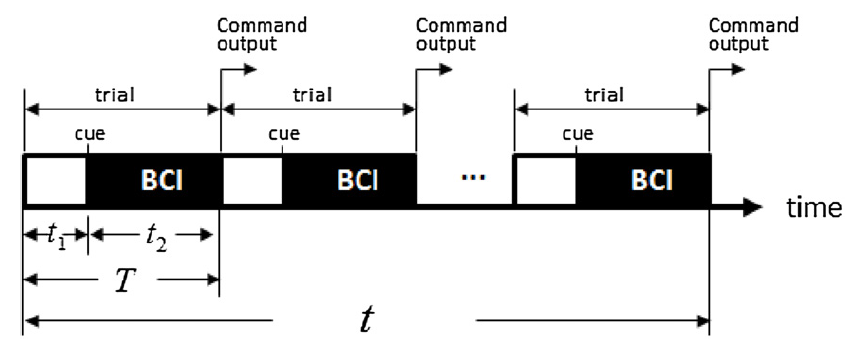
\includegraphics[width=1\textwidth]{timingBCI.PNG} 
                \caption{Timing of symbol recognition and activation}\label{itr-timing}
            \end{figure}

            By collecting several timing data points for each participant, the goal is to draw a regression graph between the age of the participants and the mean timinig for each visual cue. By calculating the statistical significance of the correlation, which was discussed in section \ref*{doe}, the hypothesis can be proven or rejected.

    \chapter{Survey Contents}\label{survey-contents}

        Chapter \ref{survey-framework} established the theoretical framework of the survey. This chapter aims to define the experiment which will be used to gather the data. To do so, the following considerations have to be made:

        \begin{enumerate}
            \item What tools will be used?
            \item How is the interface going to look like?
            \item What data will be collected?
            \item How are the age groups structured?
            \item How is the data collected?
            \item What are the questions in the questionnaire?
        \end{enumerate}

        \section{What tools will be used}

            \paragraph{Laptop with experimental application}

                A laptop will be used to conduct the study and collect the necessary timings as shown in figure \ref*{itr-timing}. This application will be used to show the user the visual stimuli in the experimental \textit{remote control interface}. This application was purposefully built with the \textit{NextMind SDK} in Unity. The timings will be collected as timestamps, which are in turn created by the application itself upon the corresponding events with a resolution down to a millisecond. The code is made available at Github\cite[]{GitHub.04102021}.

                \medskip

                In theory this experiment could be made with VR-Googles as well. This even might have a beneficial effect on the performance but due to expected technical difficulties especially for older people, this is not part of the study.

            \paragraph{NextMind BCI}                

                Shown in figure \ref*{electrodes-sensor} is the NextMind BCI, which will be used to gather the data from the VEP. The vendor provides a SDK which integrates really well in Unity and in consequence makes it easy to create a small application for the experiment with. During the experiments, this sensor will be located at the back of the participant's head, where the visual cortex is located at (figure \ref*{visual-cortex}.)

                \begin{figure}[h]     % h=here, t=top, b=bottom, p=page
                    \centering
                    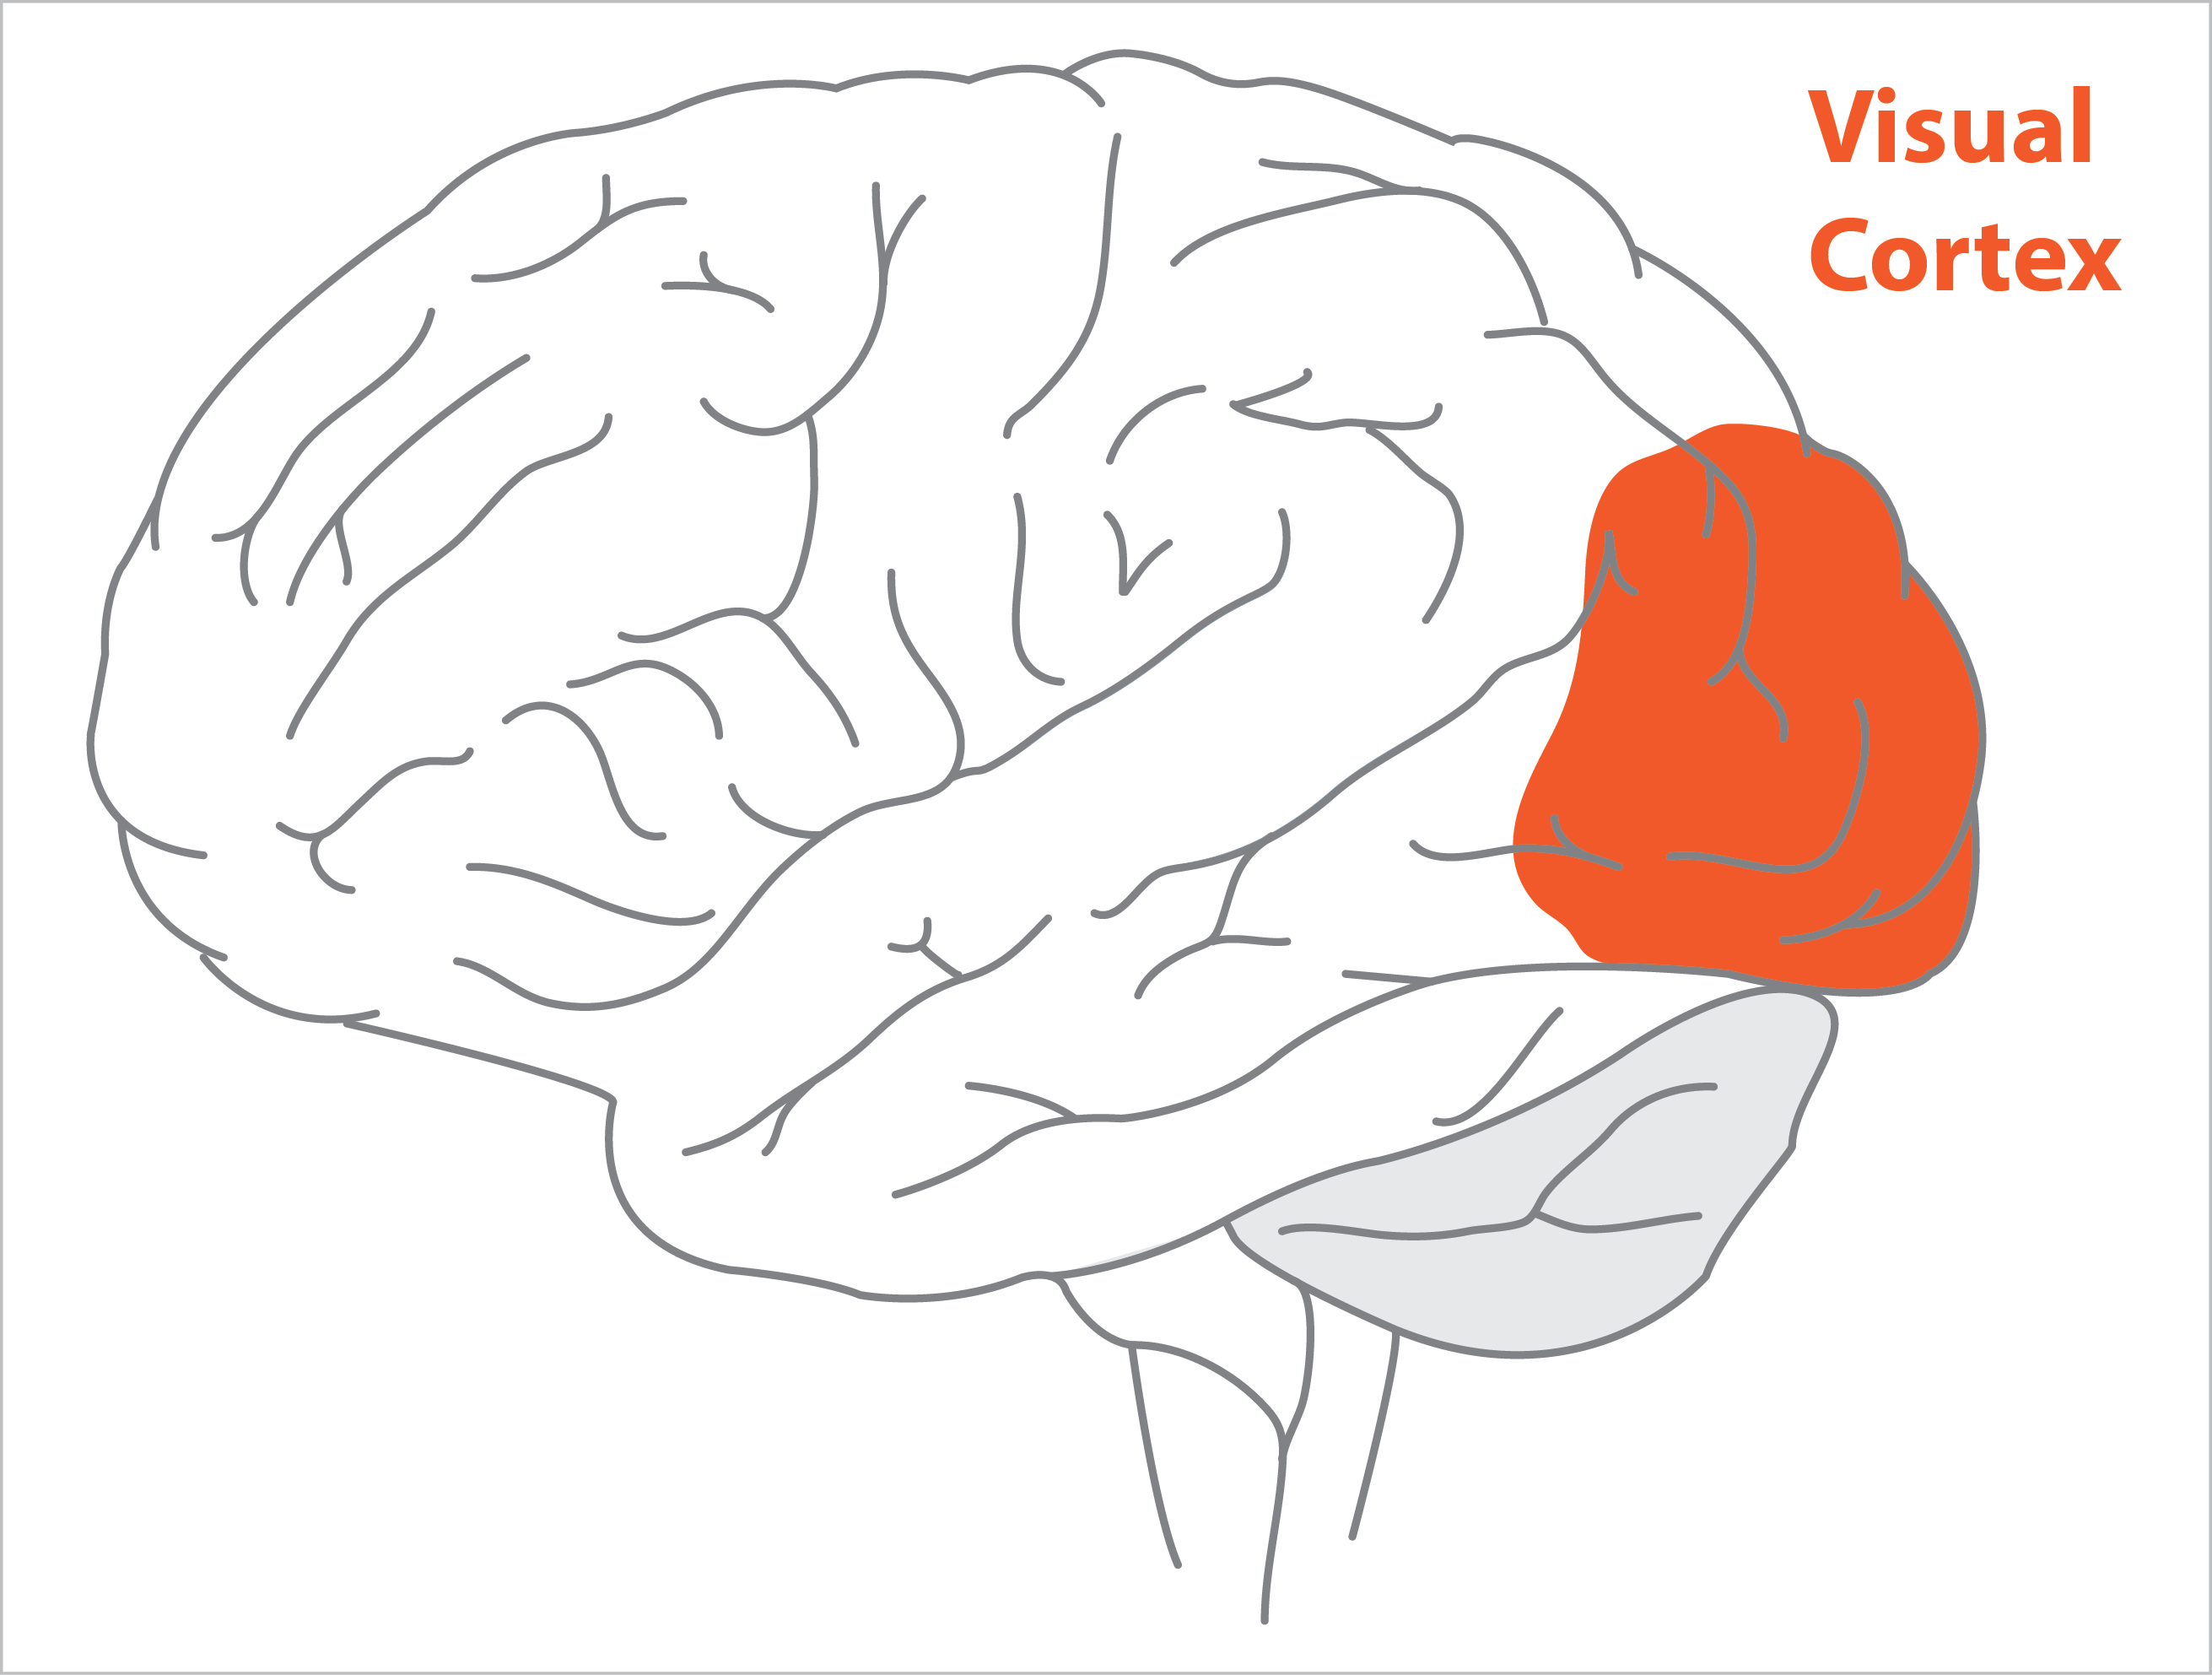
\includegraphics[width=1\textwidth]{visualcortex.png} 
                    \caption{Position of the visual cortex. Left is front. Source: \cite{Dr.KenBrodaBahm.2013}}\label{visual-cortex}
                \end{figure}

            \paragraph{Pen and paper questionnaire}

                A questionnaire will be used to collect anonymized demographic data from the participant. This is necessary for the evaluation of the results. Among demographic data and self assessments the questionnaire will also ask for opinions. See section \ref*{datacollection} for details and the full survey at section \ref*{surveys}.

        \section{Remote control interface}
        
            Figure \ref*{gui-remote} shows the interface, which the user will see in the experiment. It resembles the number pad on a conventional TV remote control in structure. The circles with the numbers will be the neurotags, which the participant has to look at. To measure the activation time, one neurotag will be visually cued - represented by the highlighted \textit{4}. As soon as this neurotag has been activated, a new visual cue will be given. The sequence for each activation will be the same for every participant. 
            
            \begin{figure}[h]     % h=here, t=top, b=bottom, p=page
                \centering
                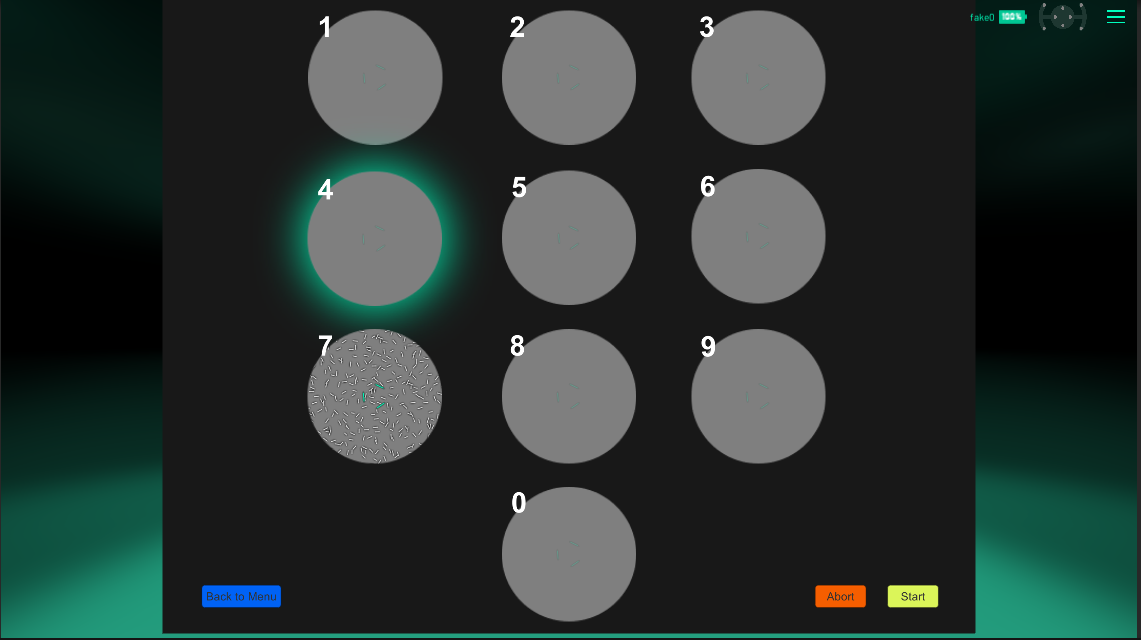
\includegraphics[width=1\textwidth]{Experiment.PNG} 
                \caption{Interface of the remote control experiment. Ques are highlighted.}\label{gui-remote}
            \end{figure} 
            
            A total of 50 different ques will be given. The order of the activation is random so there is no way the participant could know beforehand which neurotag will be cued next. Since the $t_{1}$ cannot be measured without significant effort and the absolute time is not important, it is assumed that the $t_{1}$ time for each individual is about the same for every age. Under this assumption only the $t_{2}$ will vary, which is the desired goal.

        \section{What data will be collected}\label{datacollection}

            The data collection will be structured in three blocks: Two questionnaires before and after the experiment which the participant had to answer and data collection during the experiment. The first questionnaire consisted of general questions regarding demographics and medical conditions:

            \begin{itemize}
                \item Demographics: Age and Sex
                \item If the participant wears glasses
                \item If the user felt motion sickness during the experiment
                \item Cognitive impairments
                \item Medication known to affect EEG readings
                \item Drug intake within the last 12hrs
            \end{itemize}

            The collected data during the experiment was collected on the laptop in the form of a *.csv file, which is available immediately after the experiment is finished. This data contained the following readings:

            \begin{itemize}
                \item Speed of each neurotag activation from the point where a cue was given. This is the start of $t1$ until the end of $t2$, where the sensor is confident that a certain neurotag was looked at.
                \item Confidence score of each activated neurotag upon activation until another neurotag is activated.
                \item Quality readings from each single electrode to monitor the tracking quality of the sensor, in order to explain outliers in the collected data.
            \end{itemize}
            
            After the experiment the participant answered the second block of questions, which consisted of questions about the general experience of using the BCI:
            
            \begin{itemize}
                \item If the user felt motion sickness during the experiment (rated 1...5)
                \item comfort of wearing the sensor (rated 1...5)
                \item perceived time to setup the sensor (rated 1...5)
                \item ease of use (rated 1...5) %did it work well?
            \end{itemize}           

        \section{Experimental Protocol}\label{experimental-protocol}

            The data is collected in a single session lasting between 10-20mins for each participant. Each session starts with the participant having to complete the first questionnaire \ref*{q-prior} and and the form of consent \ref*{consent} for anonymized data processing. At this stage potential hazards, problems and dispositions as discussed in section \ref{considerations} are identified.
            Afterwards each participant is introduced into the experiment. The working principle of a SSVEP is explained and questions regarding data privacy are discussed. Subsequently the GUI of the experiment is shown to the participant with a short introduction about the nature of the task.

            \begin{figure}[h]     % h=here, t=top, b=bottom, p=page
                \centering
                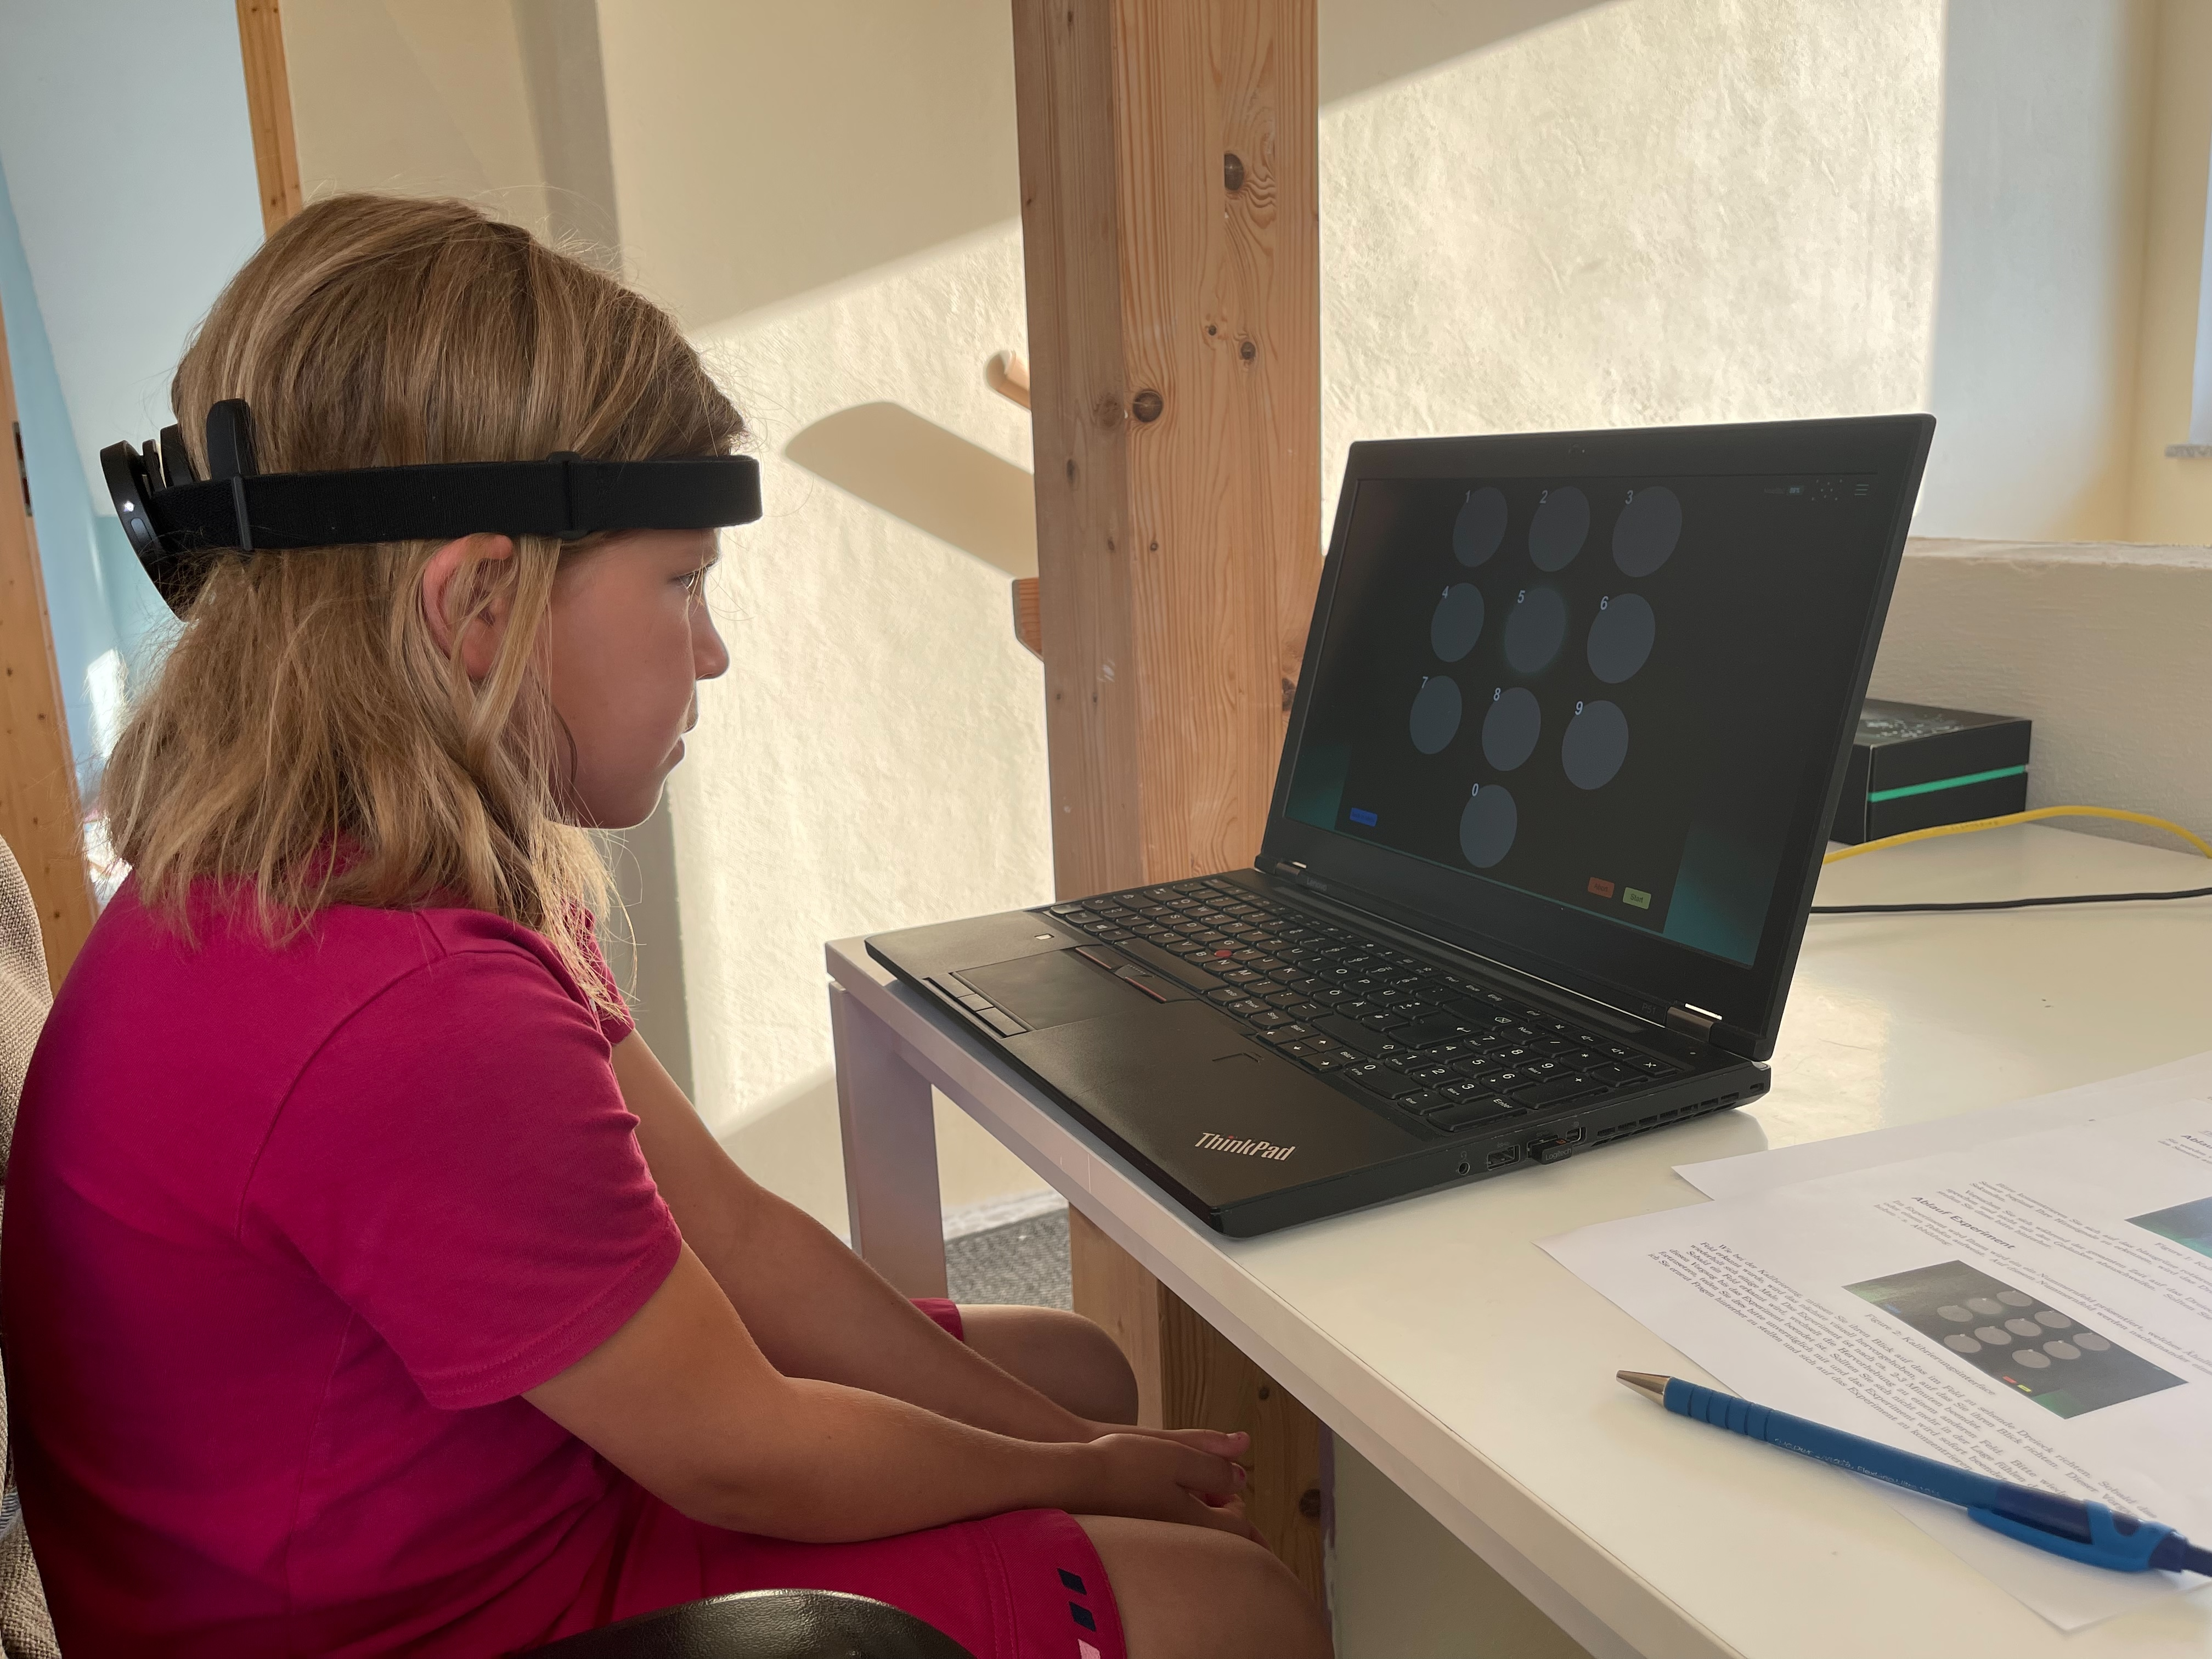
\includegraphics[width=1\textwidth]{lotta.jpg} 
                \caption{Experimental setup}\label{experimental-setup}
            \end{figure}            

            Then the participant was equipped with the BCI Sensor and placed in front of the screen as shown in figure \ref*{experimental-setup}. The distance to the screen was varying since each participant needed to adjust according to eyesight. The first step of the experiment was the calibration of the sensor to the participant. In case of non-optimal readings, the position of the sensor was adjusted accordingly until all electrodes showed at least \textit{very good} contact (figure \ref*{electrode-quality}).

            \begin{figure}[h]     % h=here, t=top, b=bottom, p=page
                \centering
                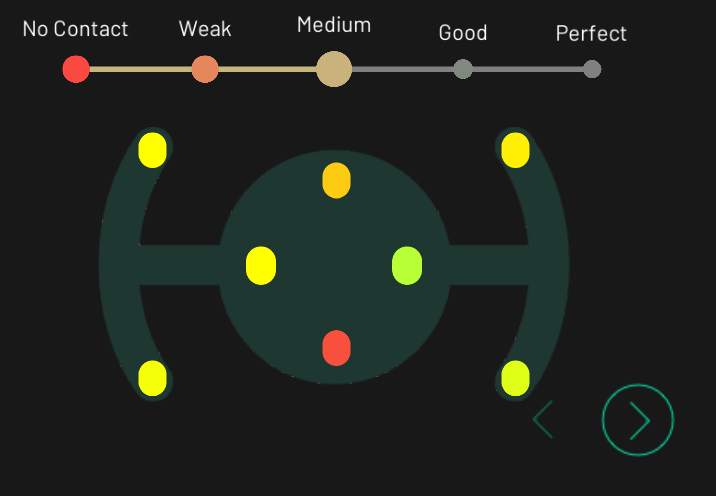
\includegraphics[width=1\textwidth]{SensorReadings.PNG} 
                \caption{Quality readings of the sensor}\label{electrode-quality}
            \end{figure}

            Then the experiment was started. The participant had to perform 50 neurotag activations. Each one consisted of a visual cue (see figure \ref*{gui-remote}) on which the participant had to focus on. Upon a sucessful activation of the cued neurotag, the readings were saved to the logfile (see \ref*{logfile}) and the next cue was given in order to keep the $t1$ timing as short as possible.

            After completion of the experiment, each participant had to fill the second questionnaire \ref*{q-post}, which gathered information about the experiment such as wearing comfort, perceived difficulty, and questions about the opinion towards the technology in general. 

    \chapter{Survey results}\label{raw-results}

        This chapter gives a brief insight into the collected data by means of visually examining them. The main focus point are the detection times for different clusterings of the population by the criteria provided by the questionnaires

        \begin{enumerate}
            \item Raw detection times
            \item Clustered by gender
            \item Clustered by glasses or no glasses
            \item Clustered by age group
            \item Clustered by different target
        \end{enumerate}

        Also the other results of the questionnaires are discussed: wellbeing, dizziness, focus, comfort, time, and perceived difficulty. Also the personal opinion and whether or not the participants found this technology useful or would use it themselves.

        \section{Raw results}

            The study gathered 1370 different target hits as datapoints from 28 participants. Figure \ref*{time-hist} shows a histogram of the achieved detection times. The y-axis is scaled logarithmically because approximately 870 out of all detections were made in under three seconds. If scaled linearly, this would have heavily skewed the overall plot. Also the occurence of detection times longer than 15-20 seconds are extremely rare in comparison.

            \begin{figure}[h]     % h=here, t=top, b=bottom, p=page
                \centering
                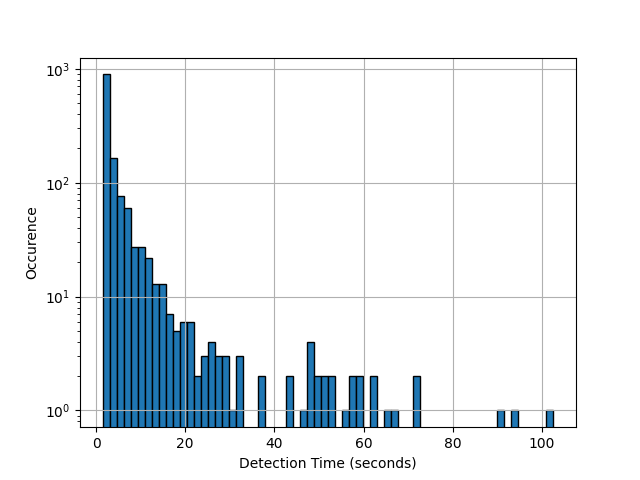
\includegraphics[width=1\textwidth]{TargetTimeHistogram.png} 
                \caption{Historgram of achieved detection times}\label{time-hist}
            \end{figure}    
            
            This is also shown very clearly in figure \ref*{time-hist-narrow}, where the time window shows only the results between two and ten seconds, which also constitutes for the majority of data points (over 95\%). Some outliers where the detection took over 120s, were removed from the sample. The clustering of the detection right at the 2.3s mark, which is indicated by the red line with almost no other data points below that threshold might indicate, that this threshold is the minimum amount of time required to confidently identify a target. The logfiles show that a confidence score of >0.3 qualifies for a successful identification. See Appendix \ref*{logfile} for details. This score is not displayed for targets, which are identified under a certain amount of time, since there aren't enough samples supposedly.

            \begin{figure}[h]     % h=here, t=top, b=bottom, p=page
                \centering
                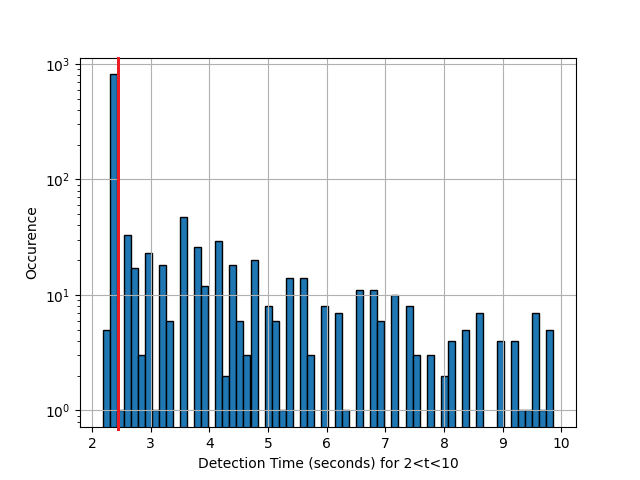
\includegraphics[width=1\textwidth]{TargetTimeHistogram_narrow.png} 
                \caption{Narrowed window of achieved detection times \todo{Occurence [log s], Move Red Line}}\label{time-hist-narrow}
            \end{figure} 

            The fact that most of the detection times center around that value might also be an identification that ~2.3s is the minimal achievable time by the BCI in conjunction with the SDK on that particular test setup. In order to have a sufficient certainty without too much noise, it is reasonable to assume that the confidence value has to be above the 90\% threshold for a defined timeframe in order to qualify for a positive detection.

            \begin{figure}[h]     % h=here, t=top, b=bottom, p=page
                \centering
                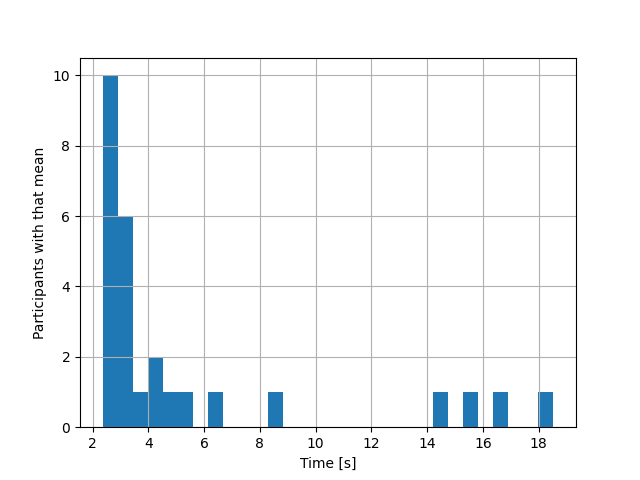
\includegraphics[width=1\textwidth]{MeanDistribution.png} 
                \caption{Achieved mean times per participant histogram}\label{mean-dist}
            \end{figure} 

            If put into perspective, figure \ref*{mean-dist} shows the same distribution but with mean times for every participant as histogram. What this data shows is that the few outliers in the achieved detection times are likely caused by a few individuals and the the majority of the participants had a very consistent timing below 10s and more so close to the minimal achieveable timing of about 2.3 seconds.

            \begin{figure}[h]     % h=here, t=top, b=bottom, p=page
                \centering
                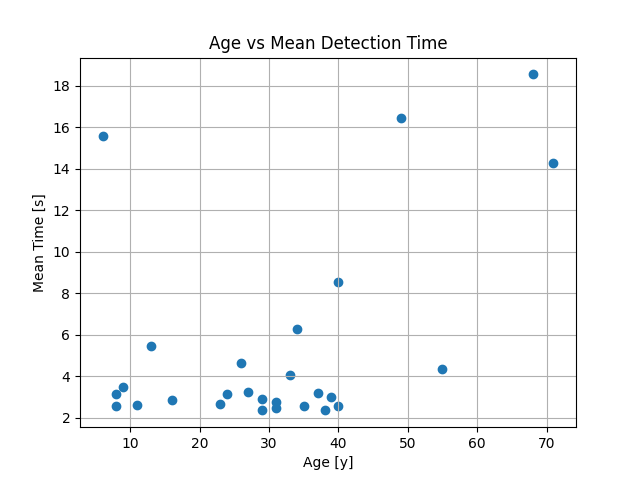
\includegraphics[width=1\textwidth]{TimesScatter.png} 
                \caption{Mean detection times plotted against age}\label{time-scatter}
            \end{figure} 

            This gets even clearer, when the mean times for each individual are shown in context to each other with the age dimension added. Conclusively what these results clearly show is that the majority of the participants who were younger than 40 showed a very consistent timing at or close to the minimum time.

        \section{Telemetry}

            The \textit{NextMind} Engine provides telemetry readings on request. Figure \ref*{telemetry} shows a boxplot of all quality readings prior to all successful conducted experiments. Each boxplot stands for one distinct electrode at the sensor. The scale is \textit{Worst to Best} in the typical \textit{Red to Green} convention with the indicated steps in between. The SDK provides a readout with a score from 0...100. 

            \begin{figure}[h]     % h=here, t=top, b=bottom, p=page
                \centering
                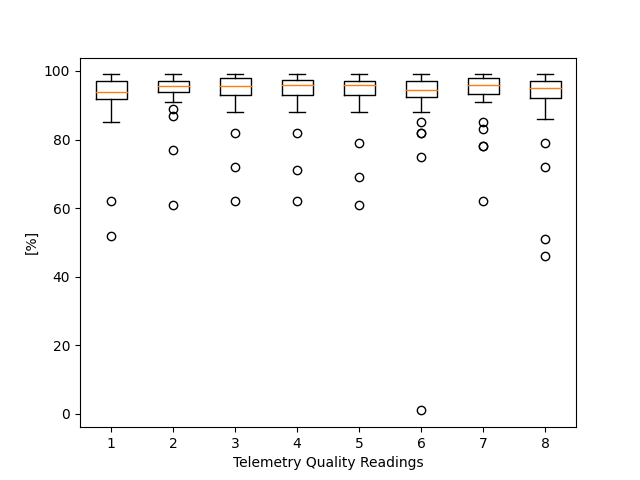
\includegraphics[width=1\textwidth]{telemetry.png} 
                \caption{Quality readings of the sensor prior to the experiments}\label{telemetry}
            \end{figure} 
            
            Apart from some outliers, there are no significant systematic errors, which might cause a significant error in the acquired data. There is a very small tendency in the outermost electrodes to have slightly less quality over the course of the whole experiment what can be attributed to being the outer and bottom electrodes which might not have ideal contact on an individual basis if the skull shape is more elliptical than usual. 

        \section{Demographic differences}\label{demographic-differences}

            To rule out potential side effects, the first questionnaire required answers for gender, whether the participant wears glasses, has neurological conditions or colourblindness, or uses alcohol or drugs, and colourblindness. However the latter four questions were answered negative entirely. The only exception was a neurological condition which resulted in the experiment not being conducted altogether in that particular case. This leaves the gender and if the participant wears glasses as the only major demographic parametres.
            
            When the genders are compared side by side in figure \ref*{gender}, there is a tendency of women having a more consistent timing. The average value of both is approximately on the same level but the male results have a larger upper quartile and whisker therefore being less consistent in timing. As in figure \ref*{time-hist-narrow}, the window was narrowed down to 10s max, to cut large outliers. However since the age distribution across genders is about the same, this won't have an effect on the outcome in regards to the hypothesis. Nevertheless a quantitative study with a large number of participants could prove if there actually is a significant effect on detection times.

            \begin{figure}[h]     % h=here, t=top, b=bottom, p=page
                \centering
                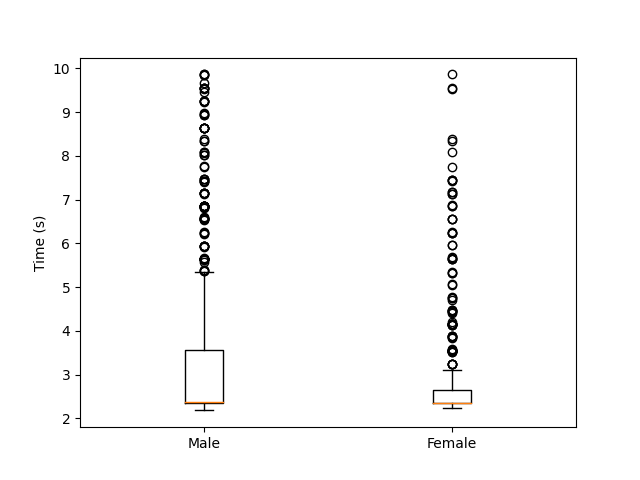
\includegraphics[width=1\textwidth]{gender.png} 
                \caption{Detection times between male and female participants}\label{gender}
            \end{figure} 

            Figure \ref*{glasses} also shows the result that participants without glasses have a higher consistency in their target times. Although the average being at roughly the same level, the upper quartile and whisker is far more spread with the participants who are wearing glasses. Since the participants which were wearing glasses tend to be about 10 years older in average than their non-glass wearing counterparts, this effect seems to be tied to the age itself and not the fact the participants actually cannot see as good.

            \begin{figure}[h]     % h=here, t=top, b=bottom, p=page
                \centering
                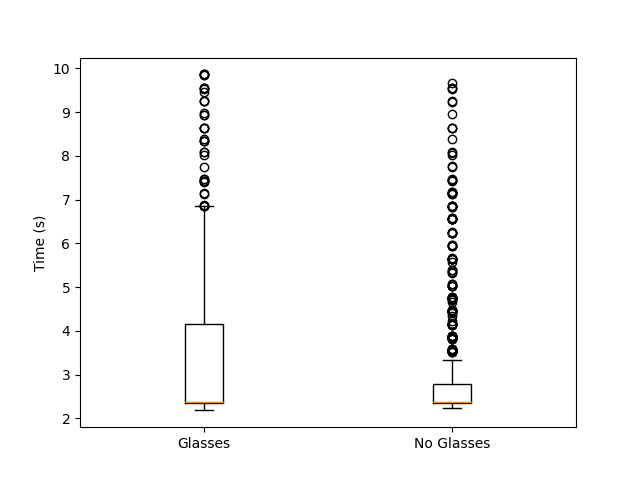
\includegraphics[width=1\textwidth]{glasses.png} 
                \caption{Detection times between participants with and without glasses}\label{glasses}
            \end{figure}

            In order to have a better understanding of the difference between younger and older participants, the whole population of the study has been binned into three different age groups:

            \begin{itemize}
                \item 0-30
                \item 31-60
                \item >61
            \end{itemize}

            The results are show in figure \ref*{age-groups}. The most prominent feature is the age group above 61 years old. Their average time to detection of the target is between 5 and 7.5 seconds. However almost indistinguishable from the 0-30 age group is the 31-60 age group but on a close look the graph actually shows a slightly slower detection time here as well. So the first preliminary finding is that there in fact is a tendency that with increasing age the detection of a target takes longer.

            \begin{figure}[h]     % h=here, t=top, b=bottom, p=page
                \centering
                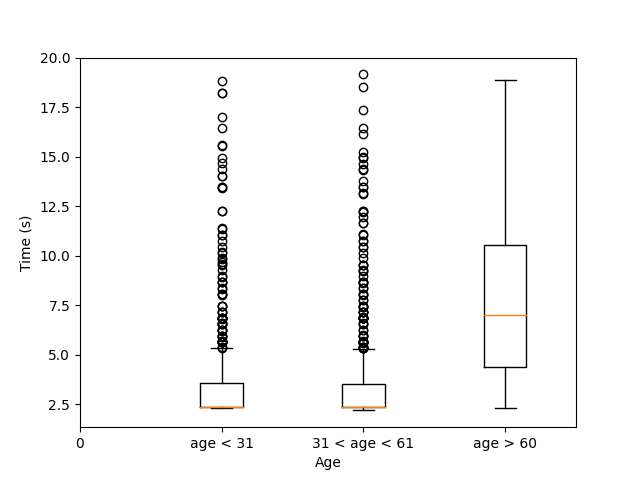
\includegraphics[width=1\textwidth]{timeDistributiion.png} 
                \caption{Detection times for three age groups}\label{age-groups}
            \end{figure}

            These results will be later set into context with other results from the survey to show a clear picture of the findings of this study.

        \section{Detection time differences for each target}

            One effect observed during the experiment was that some targets were generally faster detected than others. Figure \ref*{targets} shows this phenomennon:

            \begin{figure}[h]     % h=here, t=top, b=bottom, p=page
                \centering
                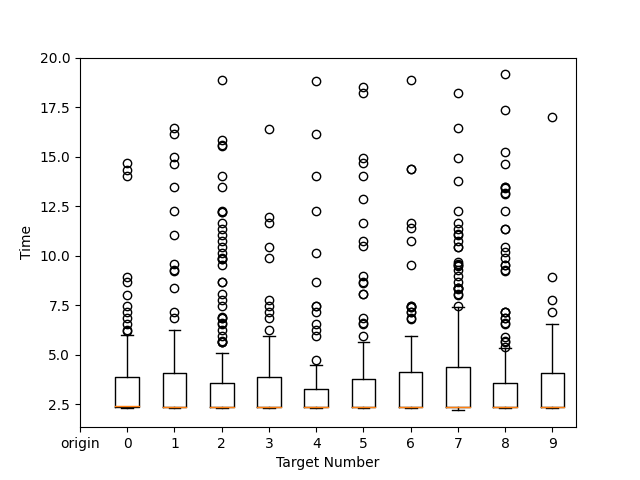
\includegraphics[width=1\textwidth]{targets.png} 
                \caption{Detection times for the different target}\label{targets}
            \end{figure}

            This effect comes presumably from the layout of the experiment itself, where the participant sat in front of a laptop and the interface was placed in a different angle. Therefore the targets, which were arragend in rows and columns (see figure \ref*{gui-remote}), were being seen in different angles. Since the test series of cues was the same for each experiment and close to evenly distributed in their occurences, there is no systematic error in the experiment itself.
            
        \section{Conduction of the Survey}
            
            Two participants had not undergone the experiment itself due to an insufficient calibration score. One case was due to missing glasses for a clear view of the screen and another case had concentration problems. Both cases were in the above 60 age group. This is especially noteworthy since in section \ref*{considerations} the assumption was made that reduced eyesight does not have an influence, since glasses can be worn. This is a strong indicator that without proper visual resolution of the neurotags, the sensor does indeed not work.
            One participant also from the above 60 age group had to end the experiment prematurely due to concentration difficulties and eye strain.

            Eye strain was reported from four participants. However there was no majority among any age group in this case which means that this does not indicate a correlation. Two participants wore contact lenses. One participant reported that focusing on the experiment made her forget about blinking her eyes, causing dry eyes.

            Two participants reported that they felt the SSVEP physically inside their brain with a pulsating or tickling sensation. However, this was not reported to be painful.

            In many cases the calibration wasn't successful on first try. Usually a sufficient score was reached after 3-5 attemps. Also for some participants the optimal sensor position was in a different place on the back of the skull than recommended by \textit{NextMind}. In these cases the results we perfect instantly after a relocation of the sensor to a different position.

            One participant inadvertenly altered the position of the sensor which did not have a significant effect on the detection time. Also with this same participant the calibration score was comparatively low. Although not explicitly tested in this survey, this might indicate that the \textit{NextMind} sensor has a resilient design to a shifting position. This would allow for applications which includes physical movement.

            One individual could not participate as she had epilepsy, what might have gotten triggered by the experiment.

            \begin{figure}[h]     % h=here, t=top, b=bottom, p=page
                \centering
                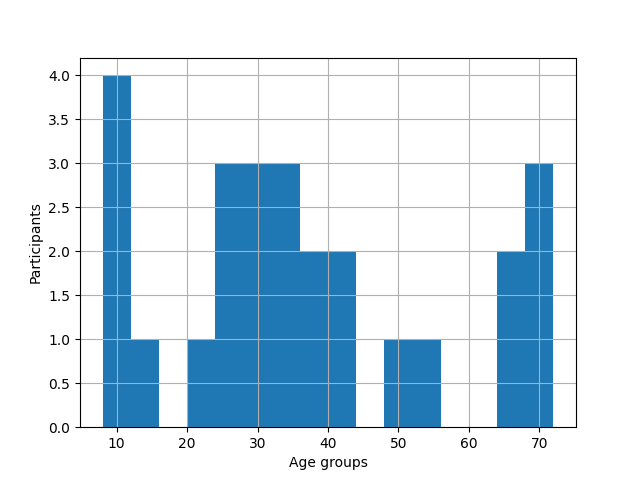
\includegraphics[width=1\textwidth]{ageDistribution.png} 
                \caption{Age distribution of the participants}\label{age-dist}
            \end{figure}

            Figure \ref*{age-dist} shows the distribution of the age of all the participants in the study. There is no age group which is particularly under- or overrepresented. The range of all participants was between 6-81 years old, resulting in a big cross section. It is noteworthy however, that not all of the participants represented in this chart also generated results for the regression curve in figure \ref*{regression}. The reason being that predominantly in the above 60 age group, some participants had problems with the calibration due to reduced eyesight or concentration problems.
     
        \section{Questionnaire Results}

            While the first survey had the primary goal to evaluate the Demographic data for the experiment and whether the subject was even able to conduct the experiment from a medical standpoint, the second survey \ref*{q-post} asked questions about the parametres of the experiment itself.

            These were:

            \begin{itemize}
                \item Wellbeing: How the participant felt that way, which might impact the ability to concentrate
                \item Dizziness: If the participant felt dizzy after the experiment
                \item Focus: How easy it was for the participant to focus on the task
                \item Comfort: The comfort of wearing the headset.
                \item Time: How the participant perceived the procedure of calibrating the sensor 
                \item Difficulty: If the task of targeting Neurotags felt difficult.
            \end{itemize}

            Figure \ref*{survey-boxplots} shows the results from the survey on a 1...5 scale. The \textbf{Wellbeing} on the day of the experiment of most participants was generally good. Only one participant had back pain, which however didn't impair the ability to concentrate. Almost no participant felt \textbf{dizziness} after the experiment. \textbf{Focus}, \textbf{Difficulty} and \textbf{Time} didn't show any noteworthy results. Interestingly there was no real tendency to the \textbf{Comfort} of wearing this sensor. The opinions about the device are very evernly distributed, which is interesting because some participants apparently found it very comfortable to wear whereas others found it really uncomfortable.

            \begin{figure}[h]     % h=here, t=top, b=bottom, p=page
                \centering
                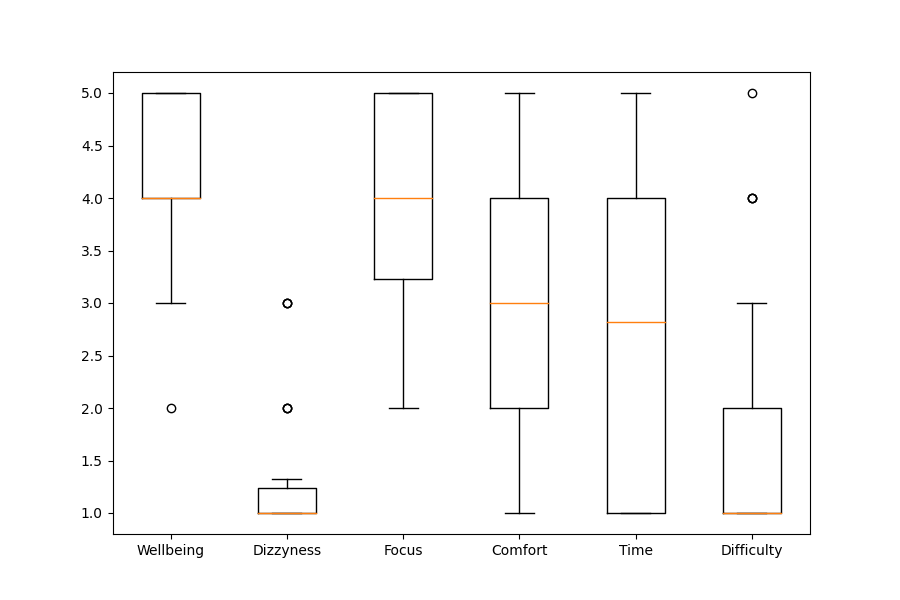
\includegraphics[width=1\textwidth]{SurveyResults.png} 
                \caption{Results of post experiment user survey}\label{survey-boxplots}
            \end{figure} 

            In terms of opinion about the technology, which is not part of this study per se but interesting to gauge a general opinion nevertheless. Only 3 out of 25 participants are sceptical towards this technology. Three persons abstained from giving an opinion and two persons didn't fill the second questionnaire. 15 out of 30 participants would use the technology themselves with the remaining 15 answers consisting of two abstentions, two not filled questionnaires and the remaining 11 being negative answers. However, 24 participants think that this technology provides a benefit in the right domain. Again two persons didn't fill the questionnaire and four refrained from answering the question.

    \chapter{Findings}\label{findings}

        \section{Age as a factor in BCI usage}\label{findings-age}

            Section \ref*{correlation} discussed, how a regression graph will be used in order to identify a trend between age and expected performance in regards to BCI usage. Figure \ref*{regression} shows the same values as figure \ref*{time-scatter} but with added regression graph and the defined 95\% confidence interval:

            \begin{figure}[h]     % h=here, t=top, b=bottom, p=page
                \centering
                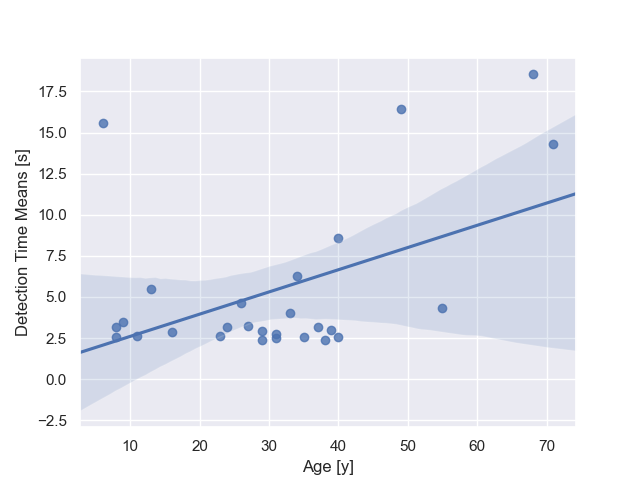
\includegraphics[width=1\textwidth]{regression_confidence.png}
                \caption{Regression graph with confidence interval}\label{regression}
            \end{figure}

            The general trend is that there in fact is a correlation between age and achieved detection times. However, taken the confidence interval into account, this result is neither clear nor definitive. If the experiment were to be repeated with the same paramenters and all the results end up within the pictured confidence interval it might very well be that new trials would in fact yield a result, where the gradient of the regression graph might be negative. Nevertheless, there are two distinct key features in figure \ref*{regression}:
            
            \paragraph{Consistency} Both younger and older people tend to be less consistent with their achieved detection times. For the younger people below the age of 20 there aren't simply enough datapoints because two outliers already skewed the resultset too much. In fact the youngest tested person with an age of six performed almost as bad as the oldest person. A possible explanation is that this participant wasn't able to concentrate on the experiment, which required dedication and focus on the task at hand. The observation of this particular participant was that he started to move around on the chair and lose focus on the task, which resulted in longer detection times. A possible explanation is that the other children were already in 3rd grade upwards and didnt have any issue with focusing on a task for a few minutes. So in this case age does have an cognitive influence but not necessarily in a way which was anticipated. 

            For older people the consistency is also spreaded more than it is within the 20-40 years range, which achieved by far the most consistent results. The reason why older people tend to deliver less consistent results for many different trials can be also attributed to the ability to concentrate for prolonged periods. In fact, if one single cue took longer to detect, this could have had a domino effect because the concentration deteriorated even faster, resulting in considerably longer detection times later on. 
            
            \paragraph{Missing Data Points} Knowing the results of the survey and the age distribution (figure \ref*{age-dist}) shows that not all participants, which are represented in the survey also participated in the experiment. The reason being that three participants in the above 40 age group had bad calibration scores and thus could not even participate in the experiment itself. Although this obviously cannot be added to the study as definitive result, it underlines the general performance of that group, where a less consistent overall performance can be expected.

        \section{Mathematical proof}\label{mafs}

            Figure \ref*{regression} already showed that within a 95\% confidence interval given enough data points, the same study should also yield results within the same range if the paramenters of the study are not altered. This section Focusses on proving that the null hypothesis holds true with the method discussed in section \ref{doe}. Figure \ref{means-density} already exhibits that there is a group of participants, whose mean timing is significantly outside of the main cluster of mean timings. From figure \ref{regression} it can also be derived that this group in fact represents the \textit{above 40 group}. The orange line printed on top is a KDF\footnote{Kernel Density Function} to highlight the influence of this group on a normalized sample.

            \begin{figure}[h]     % h=here, t=top, b=bottom, p=page
                \centering
                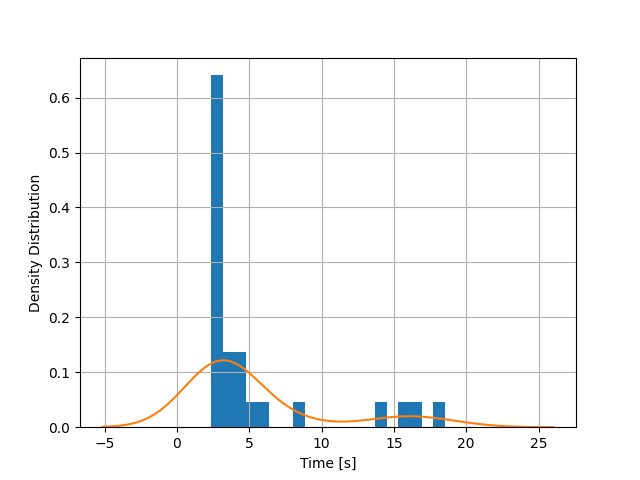
\includegraphics[width=1\textwidth]{densityDistribution.png}
                \caption{Density distribution over mean times}\label{means-density}
            \end{figure}

            In order to transform the results of collected data in the dataset to a standard normal distribution, the sample mean has to be calculated in order to later transform all parameters into a standard normal distribution. Later on, the samples means of two distinct groups will be compared to prove or reject the null hypothesis. The groups will be separated as follows:

            \begin{itemize}
                \item 0-39 years: control group - denoted as $CG$
                \item 39+ years: effect group - denoted as $EG$
            \end{itemize}

            The reason for separating the groups at this point can be seen in figure \ref{regression}: At the 40-year mark there seems to be a significant effect, which does not exist below 40 years. The sample mean however is calculated using the following equation:

            \begin{equation}\label{global-mean}
                \mu_{0} = \frac{\Sigma(\bar{X})}{n}
            \end{equation}  

            where $\bar{X}$ corresponds to the mean of any single participant's timing and $n$ corresponds to the numbers in the experiment. To calculate the standard deviation of the sample, which is required to determine the \textit{Z-Score} for any particular group, the following equation is utilized, where $\bar{X}$ is the non-normalized global mean, which was calculated previously.

            \begin{equation}\label{stddev}
                \sigma = \sqrt{\frac{\Sigma(x_{i}-\bar{x})^{2}}{n-1}}
            \end{equation}  

            With equations \ref{global-mean} and \ref{stddev} using the sample, the results are:

            \begin{itemize}
                \item $\mu_{0} = 5.37s$
                \item $\sigma = 9.11$
            \end{itemize}

            To calculate the \textit{Z-Score} for the effect group, the mean for this particular group has to be determined using equation \ref{global-mean}. This results in $\mu_{EG} = 10.7s$. Using these values, the \textit{Z-Score} for the effect group can be determined:

            \begin{equation}\label{z-value}
                Z = \frac{\mu_{EG}-\mu_{0}}{\sigma/\sqrt{n}}
            \end{equation}  

            The result is $3.11$. This means that the mean timing for the effect group is about $3\sigma$ longer than the sample mean. This in fact proves that $H_{0}$ has to be rejected and there is an effect.

            The last step is to determine the power of the experiment by calculating $\beta$. For this, we first need to calculate the threshold at which we would have rejected $H_{0}$. This is the critical $\bar{X}$ value for $2\sigma$, which is calculated using equation \ref{z-value} solved for $\bar{X}$, denoted as $\bar{X}_{critical}$ in this context:

            \begin{equation}\label{x-bar}
                \bar{X}_{critical} = \mu_{0}+\frac{\sigma}{\sqrt{n}}\times Z
            \end{equation}         
            
            Using the established values, this results in $\bar{X}_{critical} = 8.81s$. The value $\beta$ is now determined as the probability that given the established standard normal distribution, a participant of the study has a mean timing, which is larger than 8.81s. For this, equation \ref{z-value} is used again to standardize $\bar{X}_{critical}$ with $\mu_{EG}$ instead, which was established in section \ref{doe} in equation \ref{beta-probability2}. The result is $-1.11\sigma$ or a probability of 0.13. This results in a power of $P=1-\beta=0.87$ or 87\%, which is a reasonably high power assuming that this study had only results from 28 experiments.

        \section{Other findings}\label{other-findings}

            The collected dataset allowed for other interesting insights into possible performance paramenters of the participants, which were already briefly shown in the \ref*{raw-results}. This section briefly discusses these results and interpretes them in the context of this study.

            \subsection{Glasses}

                Whether the participant wears glasses or not seems to have an influence on the outcome on the performance. However, this might coincide with the fact that participants with glasses were over 10 years older in average: 30.4 years for the non-glasses group and 40.5 years for the glasses group. This is especially reasonable to assume since people tend to have more issues with eyesight the older they become.  

            \subsection{Gender}

                According to figure \ref*{gender}, there seems to be a difference between male and female participants when it comes to BCI performance. This could be an interesting starting point for further research into the \textit{why} of that anomaly. Since this study was not designed to provide an answer for this question, no further conclusion will be drawn, since it will be pure speculation. As for the influence on the dataset for this study, the survey results reflect that there is no huge age gap between the genders, which might reflect a systematic error on this side. In fact, the female participants were older with an average age of 37.3 years in comparison with the male participants with 33.2 years.

            \subsection{Target position}

                In regards to the timing for the different targets, which is shown in figure \ref*{targets}, the result is inconclusive. Although the question was raised during the conduction of the experiment, whether there it makes a difference in this setting, there weren't enough data points to prove or show a significant difference in the timings between the targets with certainty. Nor was the experiment itself structured in a way which allowed for conclusive data collection. There is also no influence on the collected data for the main objective, since every participant was shown the same experiment. Hence any systematic error would have manifested evenly across all participants if it exists.

    \chapter{Conclusion}

        \section{Results}

            Sections \ref{findings-age} and \ref{mafs} proved that in fact the hypothesis is falsified. This means that age does have an effect on the ability to use a BCI. Especially section \ref{findings-age} tried to deliver a reason for that, which is presumed to be related to the ability to concentrate on a given task for prolonged periods of time. This effect is clearly visible in the age group of 40 years onwards, according to figure \ref{regression}. Another indication is that the only two persons, who weren't able to deliver a good calibration score were also in this age group. Another interesting factor, which shows that this study had a good design, is that almost none of the participants from very young age to the oldest ones reported difficulties in the task - see figure \ref*{survey-boxplots} : Difficulty. This makes the collected dataset even more valid, because this means that there was no bias through technical difficulties.
            
            Section \ref{other-findings} used the results from the survey in order to find other reasons for this but were either not really relevant (i.e. target positions) or linked to the age (i.e. glasses). In the case of the gender, there seems to be an effect according to figure \ref{gender} but the data in this study didn't allow for further investigation.

        \section{Future Work}

            There are several ways to continue with this resarch in subsequent studies, based on the outcome of this study. These potential studies reflect on the collected results and several key points, where this study did not dive into due to the different scope. Some of them are briefly outlined in the following paragraphs:

            \paragraph{Gender} Based on the gender gap in section \ref*{other-findings}, there might be a factor in the difference in genders, which has not been discovered yet. Since there was no apparent age gap between the two genders - the female participants were in fact older - which might explain the result, there might be another factor governing this. However, the results were inconclusive. Therefore a quantitative study to reveal a systematic influence might be worthwhile. 

            \paragraph{Quantitative Study} This study could be expanded into a quantitative study in order to gain a deeper understanding of what the drivers are behind the influence of age. Especially since the ability to concentrate might have an influence here as well. A larger number of participants in the order of around a few thousand individuals very likely will draw a clearer picture of potential causes. The questionnaire could be improved as well to gain a better understanding of the process and learning curve of each individual. 

            \paragraph{Positions} Briefly discussed in the results and findings was the subject of a potential influence of the target positions. Especially in regards to a potential required movement of the head in order to focus on new cues. This will very likely increase the $t_{1}$ time - see section \ref*{correlation}. An approach, where the target positions are varied across a wide range of different positions might exhibit different results in regards to timing. This also has some relevance to theoretical applications in controlling machinery or large interfaces - see section \ref*{beyond} for details.

            \paragraph{Learning} One factor, which this study was not able to collect a sufficient amount of data on, was the learning progress of different participants. During the conduction of the experiment it was subjectively observed that the reaction times for each participant were faster in the later cues of the whole experiment compared to the earlier ones. However the data was inconclusive due to a high noise in the dataset for differen individuals. A potential study could evaluate if for smaller subsequent cues the participant learns to use the interface on a cognitive level and has shorter average detection times on subsequent trials.

            \paragraph{Other demographic factors} Section \ref*{demographic-differences} discussed the answers to different demographic factors, which might have had a systematic influence on the results. Apart from the necessity to wear glasses and the gender, there were no participants providing a different than negative answer. Nevertheless, it would be interesting to see whether colourblindness, intoxication or medication would result in different performance. Especially caffeine consumption as a popular neurological effective drug might be worthwhile to examine. 

    \chapter{Acknowledgements}

        I want to thank Prof. Dr. Roland Greule and Dipl. Inf. Rüdiger Höfert to examine this study and always set the right impulses to guide the outcome of this thesis. Rüdiger Höfert in particular helped me out with the procurement of necessary equipment to conduct the study. I also want to express my gratitude to the Hamburg University of Applied Sciences to provide the necessary framework to obtain my degree and aid with the procurement of necessary equipment. I also want to express my appreciation for every single participant who took part in my experiments despite certain constraints due to the Covid19 pandemic.
        A special thanks goes to B.Sc. Moritz Bednorz, who helped me sharpen and clarify my knowledge in the field of medical engineering and design of experiment, which gave this thesis a coherent perspective on all domains. 
        I will be eternally grateful to my father Dr. Thomas Neudecker to set the right impulses which made pursue an academic degree. He may rest in piece. 
        My biggest thanks is dedicated to my girlfriend B.A. Alexandra Michels for her emotional support and creative input to some of the figures in this thesis.

    \appendix

        \chapter{Material}

            \section{Survey forms}\label{surveys}

                The following forms were used during the experiment. They are written in the german language since every participant was native german. 

                \medskip

                \textit{Every document is in its original layout, hence the difference in terms of layout to the rest of this document.}


                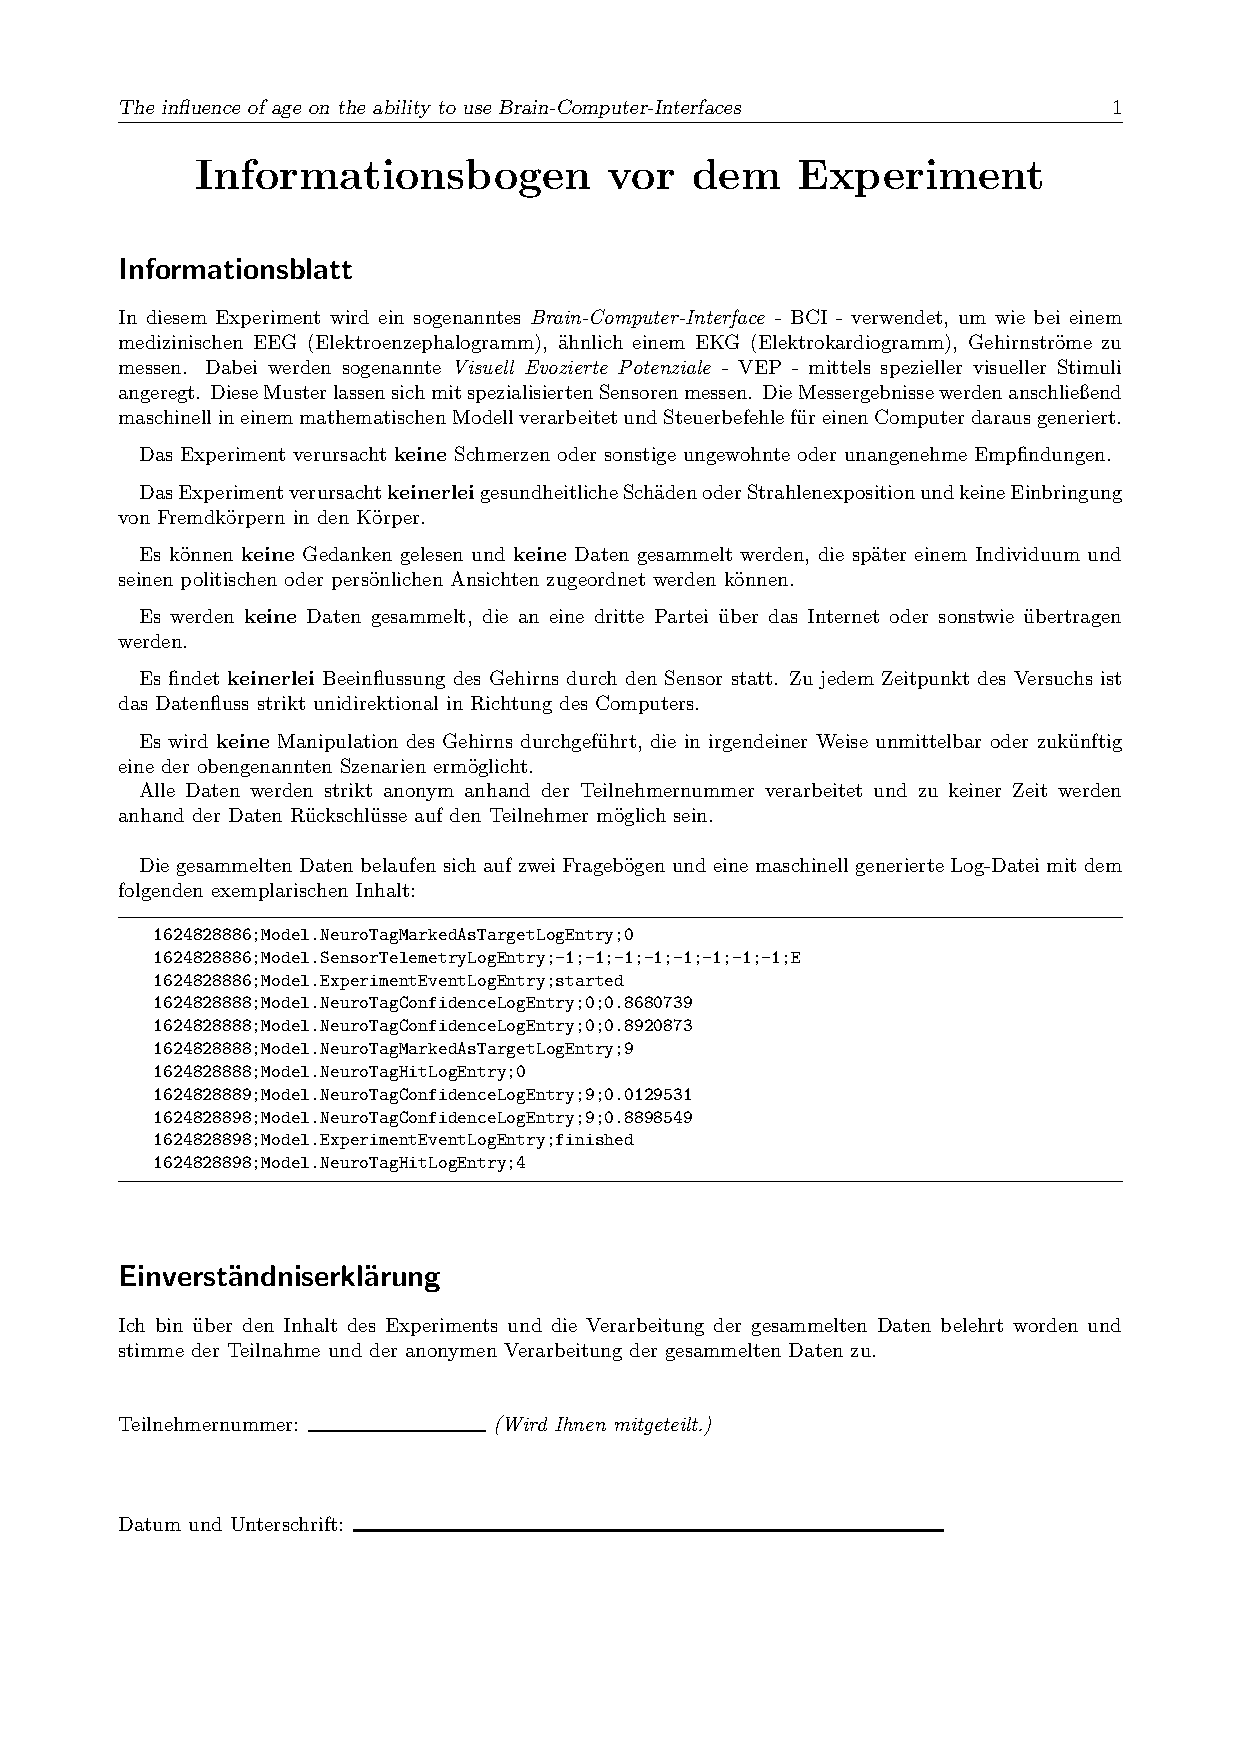
\includepdf[fitpaper=true, pages=-]{InfoSheetAndConsent.pdf}\label{consent}
                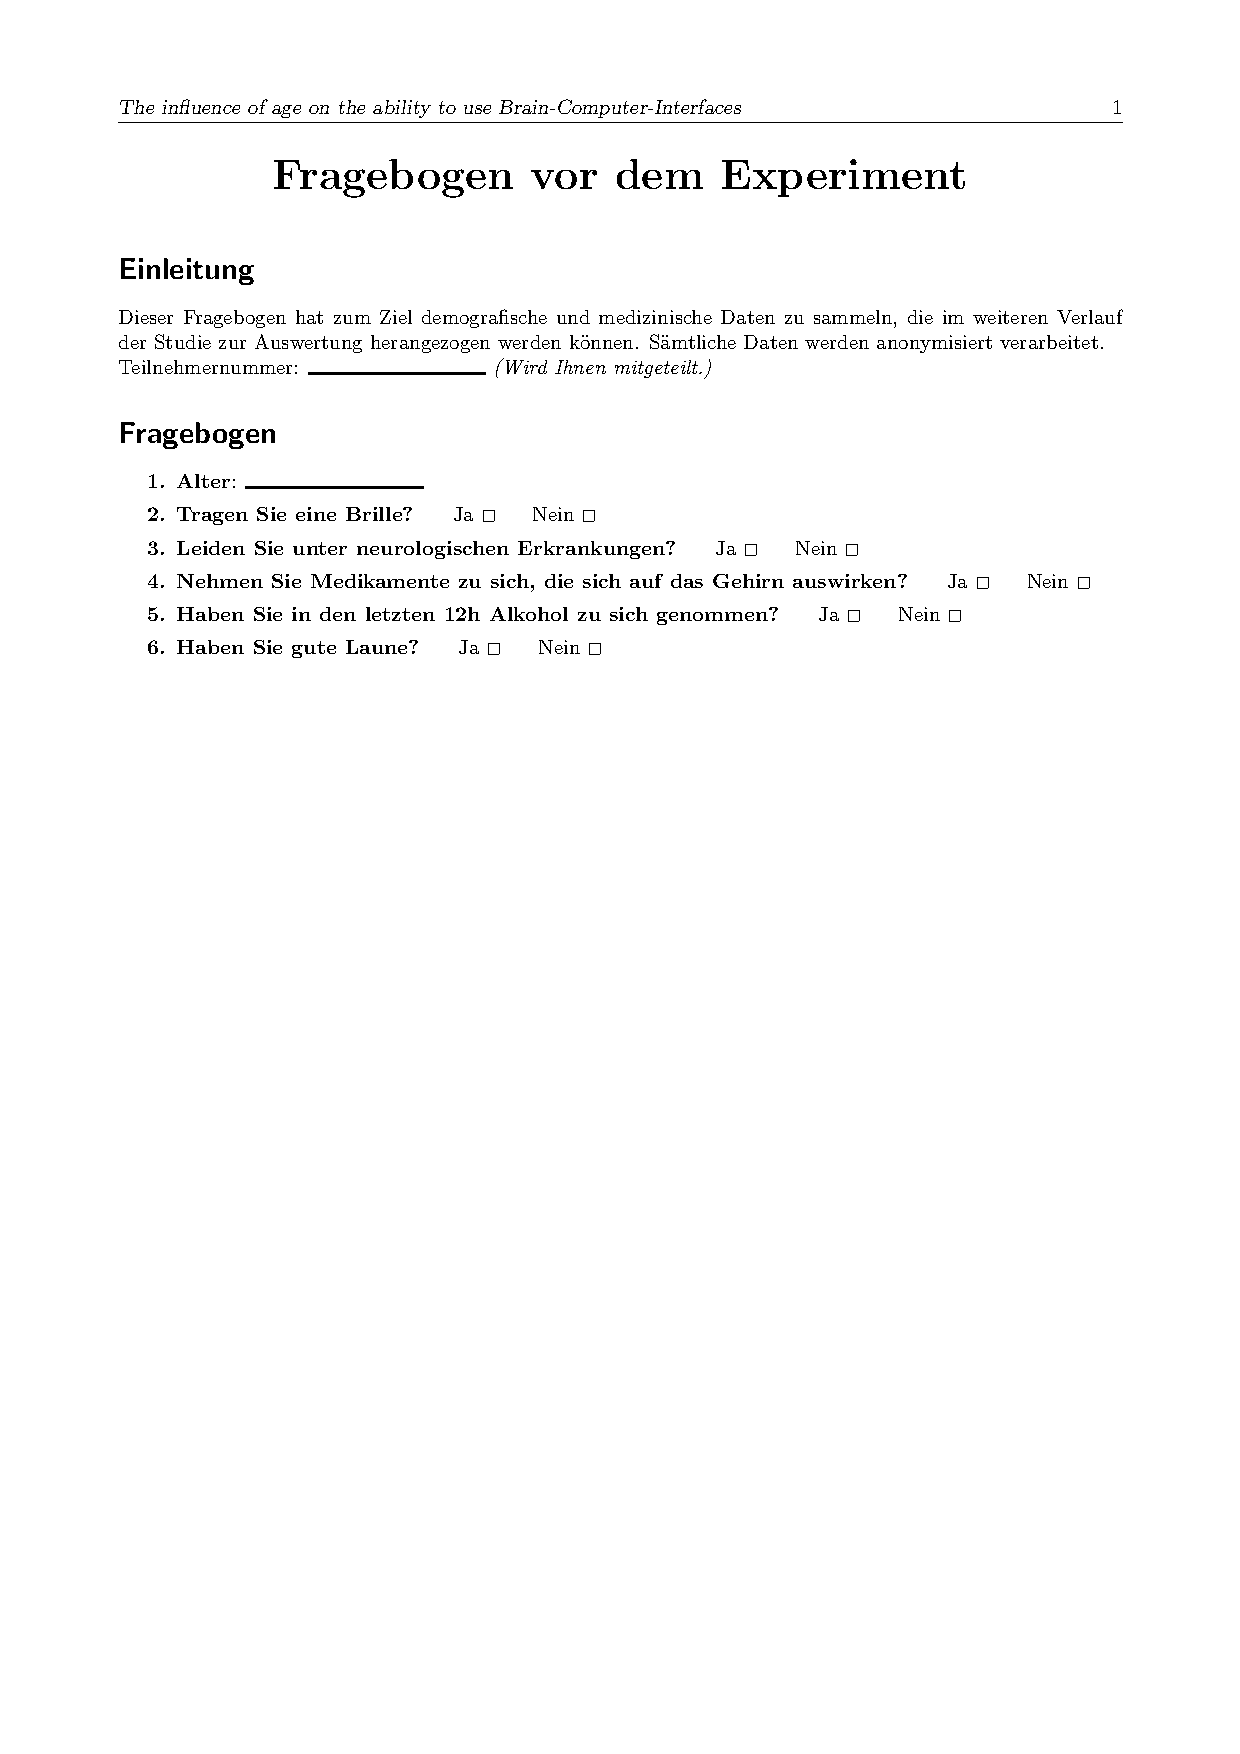
\includepdf[fitpaper=true, pages=-]{Questionnaire-Prior.pdf}\label{q-prior}
                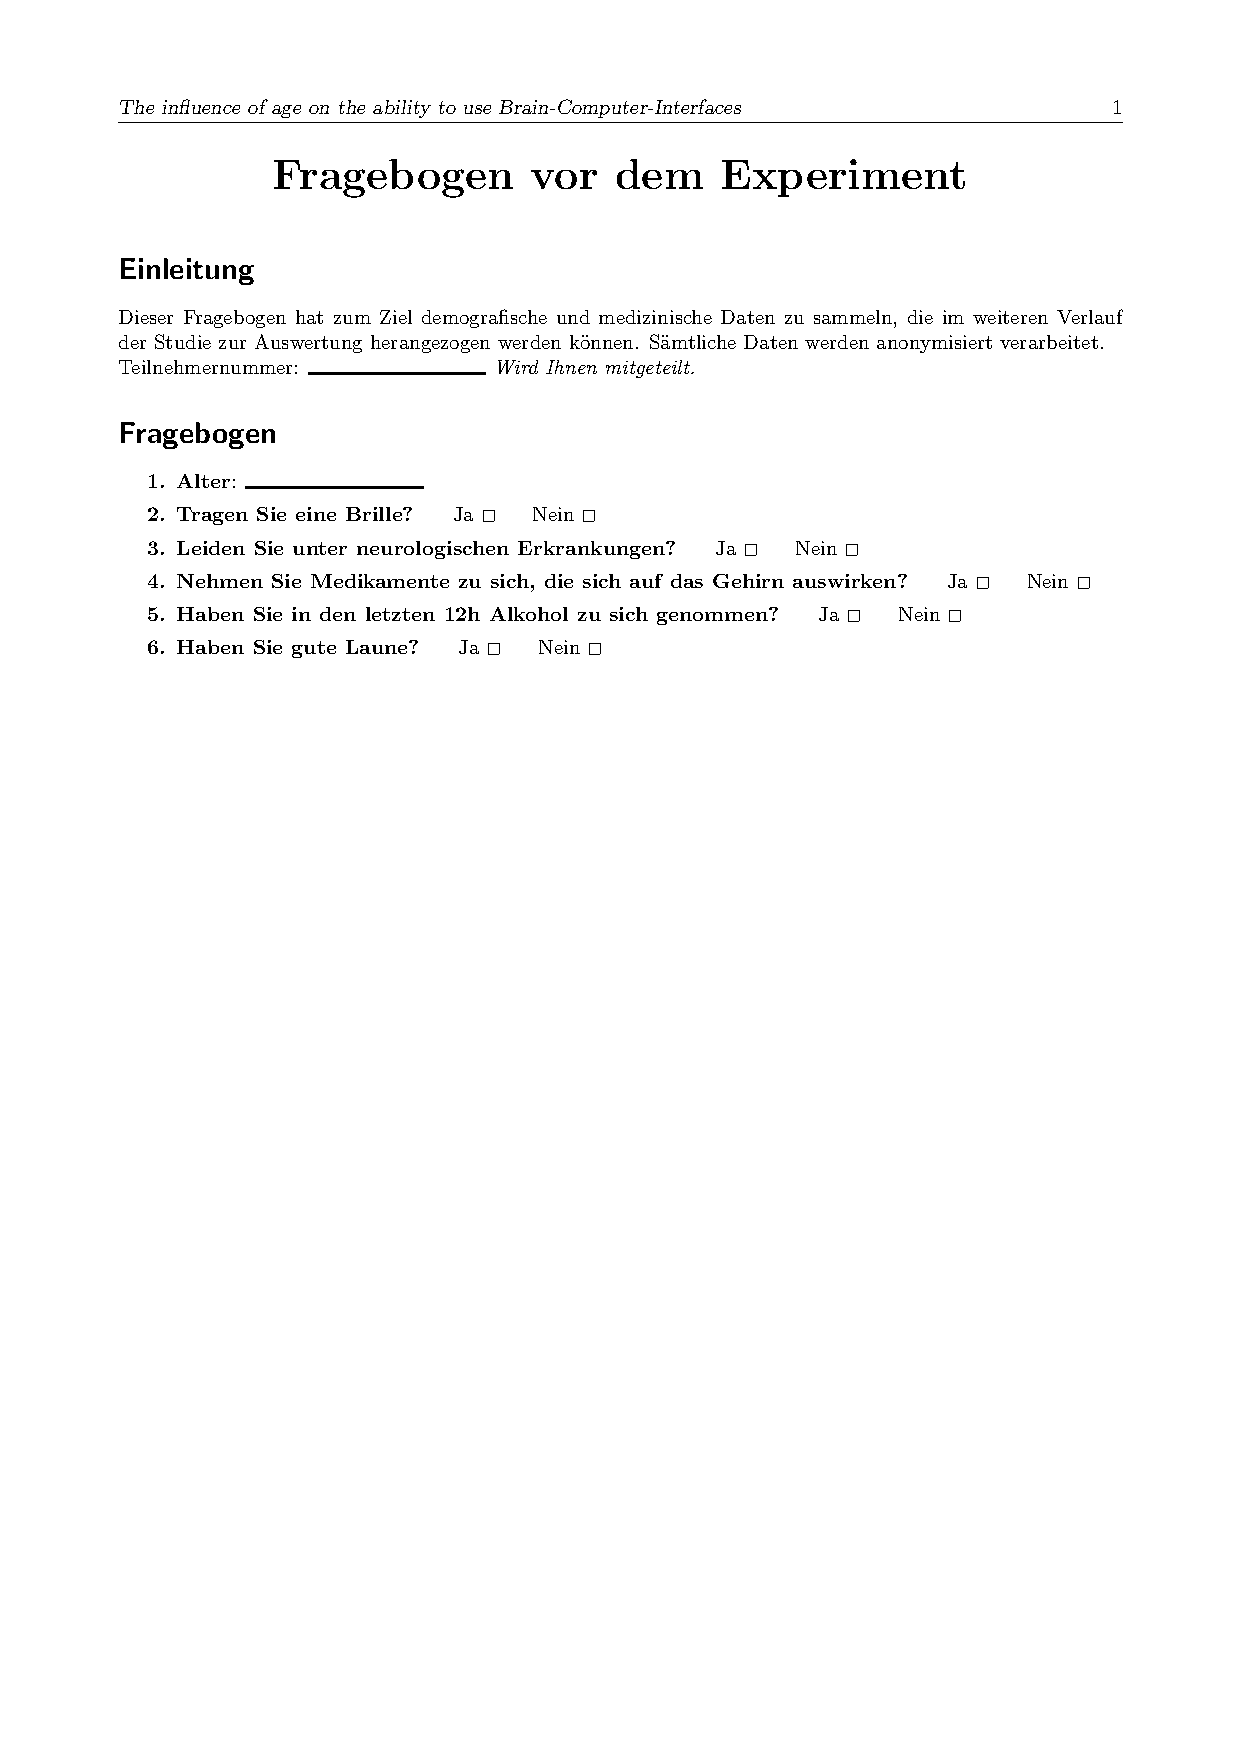
\includepdf[fitpaper=true, pages=-]{Questionnaire-Post.pdf}\label{q-post}

            \section{Example logfile}\label{logfile}                

                This is an excerpt of a genuine logfile and shows all the relevant data which was gathered during a trial. 
                
                \medskip

                \textit{Since the data is anonymized, there is no way to identify a certain individual from this excerpt.}

                \begin{lstlisting}
                    1626361044463;Model.NeuroTagMarkedAsTargetLogEntry;7
                    1626361044468;Model.SensorTelemetryLogEntry;94;95;94;93;93;85;97;94;C
                    1626361044468;Model.ExperimentEventLogEntry;started
                    1626361044559;Model.NeuroTagConfidenceLogEntry;7;0.03284512
                    1626361044858;Model.NeuroTagConfidenceLogEntry;7;0.02825086
                    1626361045158;Model.NeuroTagConfidenceLogEntry;7;0.04584821
                    1626361045458;Model.NeuroTagConfidenceLogEntry;7;0.0324579
                    1626361045758;Model.NeuroTagConfidenceLogEntry;7;0.1790879
                    1626361046075;Model.NeuroTagConfidenceLogEntry;7;0.2322663
                    1626361046374;Model.NeuroTagConfidenceLogEntry;7;0.2289219
                    1626361046658;Model.NeuroTagConfidenceLogEntry;7;0.2858692
                    1626361046958;Model.NeuroTagConfidenceLogEntry;7;0.2982492
                    1626361047258;Model.NeuroTagMarkedAsTargetLogEntry;2
                    1626361047259;Model.NeuroTagHitLogEntry;7
                    1626361049623;Model.NeuroTagMarkedAsTargetLogEntry;9
                    1626361049623;Model.NeuroTagHitLogEntry;2
                    1626361051955;Model.NeuroTagMarkedAsTargetLogEntry;8
                    1626361051955;Model.NeuroTagHitLogEntry;9
                    1626361054287;Model.NeuroTagMarkedAsTargetLogEntry;7
                    1626361054287;Model.NeuroTagHitLogEntry;8
                    1626361054287;Model.NeuroTagConfidenceLogEntry;7;0.07452609
                    1626361056636;Model.NeuroTagMarkedAsTargetLogEntry;1
                    1626361056636;Model.NeuroTagHitLogEntry;7
                    1626361058985;Model.NeuroTagMarkedAsTargetLogEntry;2
                    1626361058986;Model.NeuroTagHitLogEntry;1
                    1626361061335;Model.NeuroTagMarkedAsTargetLogEntry;7
                    1626361061335;Model.NeuroTagHitLogEntry;2
                    1626361061335;Model.NeuroTagConfidenceLogEntry;7;0
                    1626361063699;Model.NeuroTagMarkedAsTargetLogEntry;0
                    1626361063700;Model.NeuroTagHitLogEntry;7
                    1626361066049;Model.NeuroTagMarkedAsTargetLogEntry;8
                    1626361066049;Model.NeuroTagHitLogEntry;0
                    1626361066049;Model.NeuroTagConfidenceLogEntry;8;0.1005409
                    1626361068381;Model.NeuroTagMarkedAsTargetLogEntry;7
                    1626361068381;Model.NeuroTagHitLogEntry;8
                    1626361070729;Model.NeuroTagMarkedAsTargetLogEntry;6
                    1626361070729;Model.NeuroTagHitLogEntry;7
                    1626361073079;Model.NeuroTagConfidenceLogEntry;6;0.1839611
                    1626361073396;Model.NeuroTagConfidenceLogEntry;6;0.2086784
                    1626361073696;Model.NeuroTagConfidenceLogEntry;6;0.2204314
                    1626361073995;Model.NeuroTagConfidenceLogEntry;6;0.220725
                    1626361074278;Model.NeuroTagConfidenceLogEntry;6;0.2152889
                    1626361074578;Model.NeuroTagConfidenceLogEntry;6;0.1819418
                    1626361074861;Model.NeuroTagConfidenceLogEntry;6;0.225923
                    1626361075195;Model.NeuroTagConfidenceLogEntry;6;0.1962474
                    1626361075495;Model.NeuroTagConfidenceLogEntry;6;0.2939416
                    1626361075795;Model.NeuroTagMarkedAsTargetLogEntry;2
                \end{lstlisting}
            
        %--------------------- VERZEICHNISSE ----------------

        \listoffigures % Abbildungsverzeichnis erzeugen
        \listoftables % Tabellenverzeichnis erzeugen

    %--------------------- LITERATURLISTE ---------------
    % Die Einträge sollen alphabetisch sortiert sein.

    \bibliography{references} 
    \bibliographystyle{unsrtnat}

    %--------------------- EIGENSTÄNDIGKEITSERKLÄRUNG ---------------
    \clearpage\thispagestyle{empty}
    \eigen  % im header definiert
    %--------------------------------------- ENDE ------------------------------------

\end{document}